\chapter{System Verification and Experimental Results}
\label{chap:results}

\section{Experimental Design and Verification Setup}

Following Empirical Software Engineering evaluation standards~\cite{wohlin2012experimentation}, this chapter evaluates \textbf{CITRA} (\texttt{v3.90.7}) through automated unit, integration, and browser test suites, requirements traceability verification, and controlled quantitative benchmarks structured around five Research Questions (\textbf{RQ1}--\textbf{RQ5}).

\subsection{Research Questions}

\begin{itemize}
    \item \textbf{RQ1 (In-Distribution Accuracy and Ablation):} How accurately does the proposed neuro-symbolic engine classify citations on a leak-free, paper-disjoint benchmark compared with single-source, lexical, neural, and pure machine-learning baselines (\texttt{B0}--\texttt{B5})?
    \item \textbf{RQ2 (Out-of-Distribution Symbolic Robustness):} How effectively do symbolic guardrails handle discrete integrity violations (retracted papers, chimeric DOIs, placeholder URLs, regional DOIs, API rate limits, and statutory mismatches) where continuous linear classifiers fail?
    \item \textbf{RQ3 (Probability Calibration and CIS Stability):} Does logit-space Platt scaling improve confidence calibration and selective risk-coverage trade-offs, and how stable are Citation Integrity Score (CIS) manuscript rankings under rubric weight perturbations?
    \item \textbf{RQ4 (Multi-Domain and Real Manuscript Generalization):} Does the end-to-end pipeline generalize across raw multi-domain references, multi-style academic PDFs, Vietnamese legal corpora, and real undergraduate capstone reports?
    \item \textbf{RQ5 (Latency, Caching, and Concurrency Scalability):} Does the platform satisfy all non-functional latency, memory, and 50-user deadline burst SLAs on standard CPU hardware?
\end{itemize}

\subsection{Automated Test Suites and Requirements Traceability Matrix}

Software verification spans three automated test layers summarized in Table~\ref{tab:test-suites}: 2,410+ passing backend \texttt{pytest} unit and integration tests (with environment-gated live-network skips and 0 failures), 488 passing frontend \texttt{Vitest} tests across 63 suites, and 20 \texttt{Playwright} end-to-end browser specification suites across desktop, tablet, and mobile viewports. In addition, an offline retrieval test over 500 stratified ACL Anthology queries achieved $99.80\%$ recall ($499/500$) and $100.0\%$ precision at $87.62\text{\,ms}$ mean latency. Table~\ref{tab:rtm} provides the bidirectional Requirements Traceability Matrix (RTM) linking the functional and non-functional specifications from Chapter~\ref{chap:overview} to their implementing packages and verification evidence.

{\setlength{\tabcolsep}{3.5pt}
\begin{longtable}{|L{0.23}|L{0.25}|L{0.52}|}
\caption{Automated software verification suites executed in version \texttt{3.90.7}.}\label{tab:test-suites}\\
\hline
\textbf{Verification Layer} & \textbf{Execution Result} & \textbf{Verified Subsystem Scope} \\
\hline
\endfirsthead
\multicolumn{3}{c}{\itshape Table \thetable\ (continued from previous page)}\\
\hline
\textbf{Verification Layer} & \textbf{Execution Result} & \textbf{Verified Subsystem Scope} \\
\hline
\endhead
\hline
\multicolumn{3}{r}{\itshape Continued on next page}\\
\endfoot
\hline
\endlastfoot
\textbf{Backend (\texttt{pytest})} & \textbf{2,410+ passed (0 failed)} & Multi-format extraction, 12 styles, \texttt{VNLegalVerifier}, 7-method linker, FTS5 + 15 APIs, SSRF-safe URL/HTML checks, 68 symbolic rules, Platt calibration, CIS, RBAC/IDOR, migrations \texttt{0001}--\texttt{0013}, and crash recovery. \\
\hline
\textbf{Frontend (\texttt{Vitest})} & \textbf{488 passed (63 suites, 0 failed)} & Auth/OAuth flows, progressive-disclosure drawers, 6 diagnostic report views, Citation Network DAG, Remediation modal, Classroom/Admin telemetry, and $<251\text{\,kB}$ chunk guards. \\
\hline
\textbf{Browser E2E (\texttt{Playwright})} & \textbf{20 spec suites (132+ scenarios)} & Zero horizontal overflow across 5 viewports $\times$ Light/Dark $\times$ EN/VI, SSE upload, split-pane inspection, teacher override, and 404/error recovery. \\
\hline
\end{longtable}
}

{\setlength{\tabcolsep}{3.5pt}
\begin{longtable}{|L{0.18}|L{0.34}|L{0.34}|C{0.14}|}
\caption{Requirements Traceability Matrix (RTM) mapping functional and non-functional specifications to code and verification suites.}\label{tab:rtm}\\
\hline
\textbf{Req.\ IDs} & \textbf{Implementing Modules} & \textbf{Verification Suite / Benchmark} & \textbf{Status} \\
\hline
\endfirsthead
\multicolumn{4}{c}{\itshape Table \thetable\ (continued from previous page)}\\
\hline
\textbf{Req.\ IDs} & \textbf{Implementing Modules} & \textbf{Verification Suite / Benchmark} & \textbf{Status} \\
\hline
\endhead
\hline
\multicolumn{4}{r}{\itshape Continued on next page}\\
\endfoot
\hline
\endlastfoot
\texttt{FR-01}, \texttt{FR-02}, \texttt{NFR-06} & \texttt{api/routes/auth.py}, \texttt{routes/users.py}, \texttt{link\_validator.py} & RBAC/IDOR, SSRF pinned-IP, \& \texttt{bcrypt}/SHA-256 auth tests (\texttt{pytest} + \texttt{Playwright}) & Pass ($100\%$) \\
\hline
\texttt{FR-03}, \texttt{FR-04}, \texttt{NFR-03}, \texttt{NFR-04} & \texttt{api/routes/essays.py}, \texttt{api/progress.py}, \texttt{api/job\_recovery.py} & Magic-byte, CAS quota refund, \& 50-user burst stress suite (Table~\ref{tab:nfr-deadline-stress}) & Pass ($50/50$) \\
\hline
\texttt{FR-05}, \texttt{FR-06} & \texttt{extraction/document\_parser.py}, \texttt{grobid\_adapter.py}, \texttt{docx\_parser.py}, \texttt{patterns/*} & 310-PDF multi-style \& VN legal corpus + 841-PDF regression suite (Table~\ref{tab:pdf-corpora}) & Pass ($97.7$--$100\%$) \\
\hline
\texttt{FR-07} & \texttt{linking/citation\_linker.py}, \texttt{duplicate\_detector.py} & Bipartite linking unit tests \& consistency E2E suite & Pass ($100\%$) \\
\hline
\texttt{FR-08}, \texttt{FR-09} & \texttt{database/local\_db.py}, \texttt{retrieval\_orchestrator.py}, \texttt{html\_meta\_verifier.py} & 500-query FTS5 benchmark ($99.8\%$ recall) \& OOD categories 1, 3, 4, 5 (Table~\ref{tab:ood-stress}) & Pass ($99.8\%$) \\
\hline
\texttt{FR-10}, \texttt{FR-11}, \texttt{NFR-05} & \texttt{matching/semantic.py}, \texttt{logic/rules.py}, \texttt{calibration.py} & 120K disjoint benchmark ($N=18\text{K}$ test) \& 2.4K OOD suite (Tables~\ref{tab:baselines}--\ref{tab:calibration-results}) & Pass ($99.67\%$) \\
\hline
\texttt{FR-12}, \texttt{FR-13}, \texttt{FR-14} & \texttt{logic/cis.py}, \texttt{docx\_exporter.py}, \texttt{routes/essays.py}, \texttt{Shared\allowbreak ReportPage.tsx} & $300 \times 20$ CIS simplex test ($\rho = 0.9987$), DOCX repair \& HMAC share tests & Pass ($100\%$) \\
\hline
\texttt{FR-15}, \texttt{FR-16} & \texttt{api/\allowbreak routes/\allowbreak teacher.py}, \texttt{routes/system.py}, \texttt{ClassDetailPage.tsx}, \texttt{SystemHealthPage.tsx} & Transactional override, cohort analytics, \& circuit-breaker tests & Pass ($100\%$) \\
\hline
\texttt{NFR-01}, \texttt{NFR-02}, \texttt{NFR-07}--\texttt{10} & Full 8-layer pipeline, Docker Compose, \& Vite build (\texttt{web/}) & Latency/RSS ($P_{90}=1.33\text{\,s}$, $1.03\text{\,GB}$), WCAG E2E, $2{,}920+$ tests, chunk \& container health checks & Pass ($100\%$) \\
\hline
\end{longtable}
}

\subsection{Benchmark Datasets and Perturbation Taxonomy}

Table~\ref{tab:dataset} summarizes the evaluation datasets constructed to test every layer without train-test contamination:
\begin{enumerate}
    \item \textbf{120,000-Sample Paper- and Title-Disjoint Benchmark:} From 128,115 valid unique papers in \texttt{local\_papers.db}, exactly 120,000 distinct papers (80,000 with full abstracts $>80$ characters and 40,000 metadata-complete records) were partitioned \emph{prior to perturbation} into \textbf{Train} (84,000, $70\%$), \textbf{Validation} (18,000, $15\%$), and \textbf{Held-Out Test} (18,000, $15\%$). Programmatic set-intersection checks confirm $\text{Train} \cap \text{Val} = \text{Train} \cap \text{Test} = \text{Val} \cap \text{Test} = \emptyset$ on both \texttt{paper\_id} and normalized title. Because \texttt{resource} entries are pre-screened deterministically at Order 0 (and evaluated end-to-end in \textbf{RQ4}), the 120,000-sample benchmark evaluates the four scholarly classes across \textbf{15 fine-grained perturbation sub-taxonomies}:
    \begin{itemize}
        \item \texttt{verified} ($36\%$, \texttt{V1}--\texttt{V4}): exact canonical citations (\texttt{V1}), colon-subtitle omissions (\texttt{V2}), arXiv-to-conference $\pm 1$-year transitions (\texttt{V3}), and paraphrased inline claims (\texttt{V4}).
        \item \texttt{suspected\_hallucination} ($30\%$, \texttt{H1}--\texttt{H4}): same-domain spliced titles/authors with zero registry hits (\texttt{H1}), spliced titles/authors with noisy low-overlap candidates (\texttt{H2}), non-existent DOI suffixes under real publisher prefixes (\texttt{H3}), and fabricated works paired with HTTP 404 dead links or RFC 2606 fake domains (\texttt{H4}).
        \item \texttt{metadata\_error} ($22\%$, \texttt{M1}--\texttt{M5}): publication year drift $\ge 2$ years (\texttt{M1}), swapped/grafted co-authors or venue mismatch (\texttt{M2}), valid DOI paired with moderately altered title (\texttt{M3}), non-DOI partial title alteration or contradicted body claims (\texttt{M4}), and multi-field drift or broken-URL domain exceptions (\texttt{M5}).
        \item \texttt{unresolved} ($12\%$, \texttt{U1}--\texttt{U2}): borderline title similarity inside $[0.40, 0.60)$ (\texttt{U1}) and upstream HTTP 429 rate-limit exhaustion or regional non-CSL DOIs (\texttt{U2}).
    \end{itemize}
    To prevent annotation shortcuts~\cite{poliak2018hypothesis}, full-abstract records are stratified across all four classes so non-zero Sentence-BERT alignment appears in every class ($P(\texttt{verified} \mid \text{score} > 0) = 54.06\%$), and all 419,109 unique strings are encoded with \texttt{all-MiniLM-L6-v2} without \texttt{np.clip} clamping.
    \item \textbf{2,400-Sample OOD Symbolic Guardrail Suite:} Six discrete edge-case categories ($6 \times 400 = 2{,}400$) generated strictly from held-out \texttt{test\_papers} covering retracted articles, chimeric real DOIs, RFC 2606 fake URLs, regional non-CSL DOIs, HTTP 429 API exhaustion, and Vietnamese statutory authority mismatches.
    \item \textbf{End-to-End Raw-Reference and Multi-Style PDF Corpora:} A 120-reference raw-string gold benchmark ($6\text{ domains} \times 20\text{ references}$ across 7 styles) plus 15 adversarial references, a 310-PDF multi-style and Vietnamese legal extraction corpus, an 841-PDF multi-institutional regression corpus, and full capstone report runs.
\end{enumerate}

{\setlength{\tabcolsep}{3.5pt}
\begin{longtable}{|L{0.35}|L{0.23}|L{0.42}|}
\caption{Summary of datasets used across quantitative and end-to-end evaluations.}\label{tab:dataset}\\
\hline
\textbf{Dataset / Corpus} & \textbf{Scale / Split} & \textbf{Evaluation Purpose} \\
\hline
\endfirsthead
\multicolumn{3}{c}{\itshape Table \thetable\ (continued from previous page)}\\
\hline
\textbf{Dataset / Corpus} & \textbf{Scale / Split} & \textbf{Evaluation Purpose} \\
\hline
\endhead
\hline
\multicolumn{3}{r}{\itshape Continued on next page}\\
\endfoot
\hline
\endlastfoot
\textbf{Paper-Disjoint Benchmark} & \textbf{120,000 citations} & 43.2K \texttt{ver.}, 36.0K \texttt{hall.}, 26.4K \texttt{meta.}, 14.4K \texttt{unr.} across 15 sub-taxonomies (\texttt{V1}--\texttt{U2}). \\
\hline
\quad Train / Val / Test Splits & \textbf{84K / 18K / 18K} & Zero paper or title overlap; fits LR ($C=0.25$), fits Platt ($a,b$), and evaluates \textbf{RQ1} \& \textbf{RQ3}. \\
\hline
\textbf{OOD Guardrail Stress Suite} & \textbf{2,400 citations} & $6 \times 400$ discrete symbolic guardrails built strictly from \texttt{test\_papers} (\textbf{RQ2}). \\
\hline
\textbf{Multi-Domain Raw Gold Suite} & \textbf{120 + 15 refs} & 6 domains $\times$ 7 citation styles + 15 adversarial cases, zero oracle metadata (\textbf{RQ4}). \\
\hline
\textbf{Multi-Style \& Regression PDFs} & \textbf{310 + 841 PDFs} & 30 VN legal, 60 hard-case, 220 11-style PDFs, plus 841-PDF parser stability suite (\textbf{RQ4}). \\
\hline
\end{longtable}
}

\subsection{Baselines, Evaluation Metrics, and Statistical Tests}

Six progressively stronger baselines are compared on the identical 18,000-sample test split: \texttt{B0} (\texttt{doi\_only}: exact DOI lookup), \texttt{B1} (\texttt{crossref}: single-registry Crossref lookup), \texttt{B2} (\texttt{fuzzy\_only}: RapidFuzz title + author Jaccard thresholds), \texttt{B3} (\texttt{embedding}: Sentence-BERT cosine threshold), \texttt{B4} (\texttt{no\_calib}: linear weighted heuristic without abstention), and \texttt{B5} (\texttt{ml\_hybrid}: pure 16-feature Multinomial Logistic Regression at $C = 0.25$ without symbolic guardrails).

Classification quality is measured by overall accuracy and unweighted Macro-Precision, Macro-Recall, and Macro-F1~\cite{Chawla2009}. Probability calibration is quantified by 10-bin Expected Calibration Error (ECE)~\cite{guo2017} in Equation~\eqref{eq:ece} and top-label correctness Brier Score~\cite{brier1950} in Equation~\eqref{eq:brier}:
\begin{equation}\label{eq:ece}
\text{ECE} = \sum_{b=1}^{B} \frac{|I_b|}{N} \bigl|\operatorname{acc}(I_b) - \operatorname{conf}(I_b)\bigr|,
\end{equation}
\begin{equation}\label{eq:brier}
\text{Brier} = \frac{1}{N} \sum_{i=1}^{N} \bigl(\hat{p}_i - \mathbb{I}[\hat{y}_i = y_i]\bigr)^2,
\end{equation}
where $B = 10$ denotes equal-width confidence bins partitioning $[0, 1]$, $I_b$ is the index set of test instances falling into bin $b$, $\operatorname{acc}(I_b)$ and $\operatorname{conf}(I_b)$ are the empirical accuracy and mean predicted confidence within $I_b$, $N = 18{,}000$ is the test set size, $\hat{p}_i$ and $\hat{y}_i$ are the predicted confidence and label for citation $i$, $y_i$ is the ground-truth label, and $\mathbb{I}[\cdot]$ is the indicator function. Pairwise accuracy differences are tested with continuity-corrected McNemar $\chi^2$ tests~\cite{dietterich1998approximate} adjusted across all six baseline comparisons via the Holm--Bonferroni step-down procedure~\cite{holm1979simple}, alongside 1,000-resample paired bootstrap $95\%$ confidence intervals~\cite{bergkirkpatrick2012empirical}, \cite{dror2018hitchhiker} and exact Clopper--Pearson binomial bounds for zero-count cells.

\section{RQ1: In-Distribution Verification Accuracy and Baseline Ablation}

Figure~\ref{fig:benchmark-charts} summarizes the quantitative empirical results across \textbf{RQ1}, \textbf{RQ2}, and \textbf{RQ3}. Table~\ref{tab:baselines} reports held-out test performance ($N = 18{,}000$) across \texttt{B0}--\texttt{B5} and the unified \texttt{Proposed} engine, while Table~\ref{tab:per-class} details per-class precision, recall, F1, and the four-class confusion rows.

\begin{figure}[H]
    \centering
    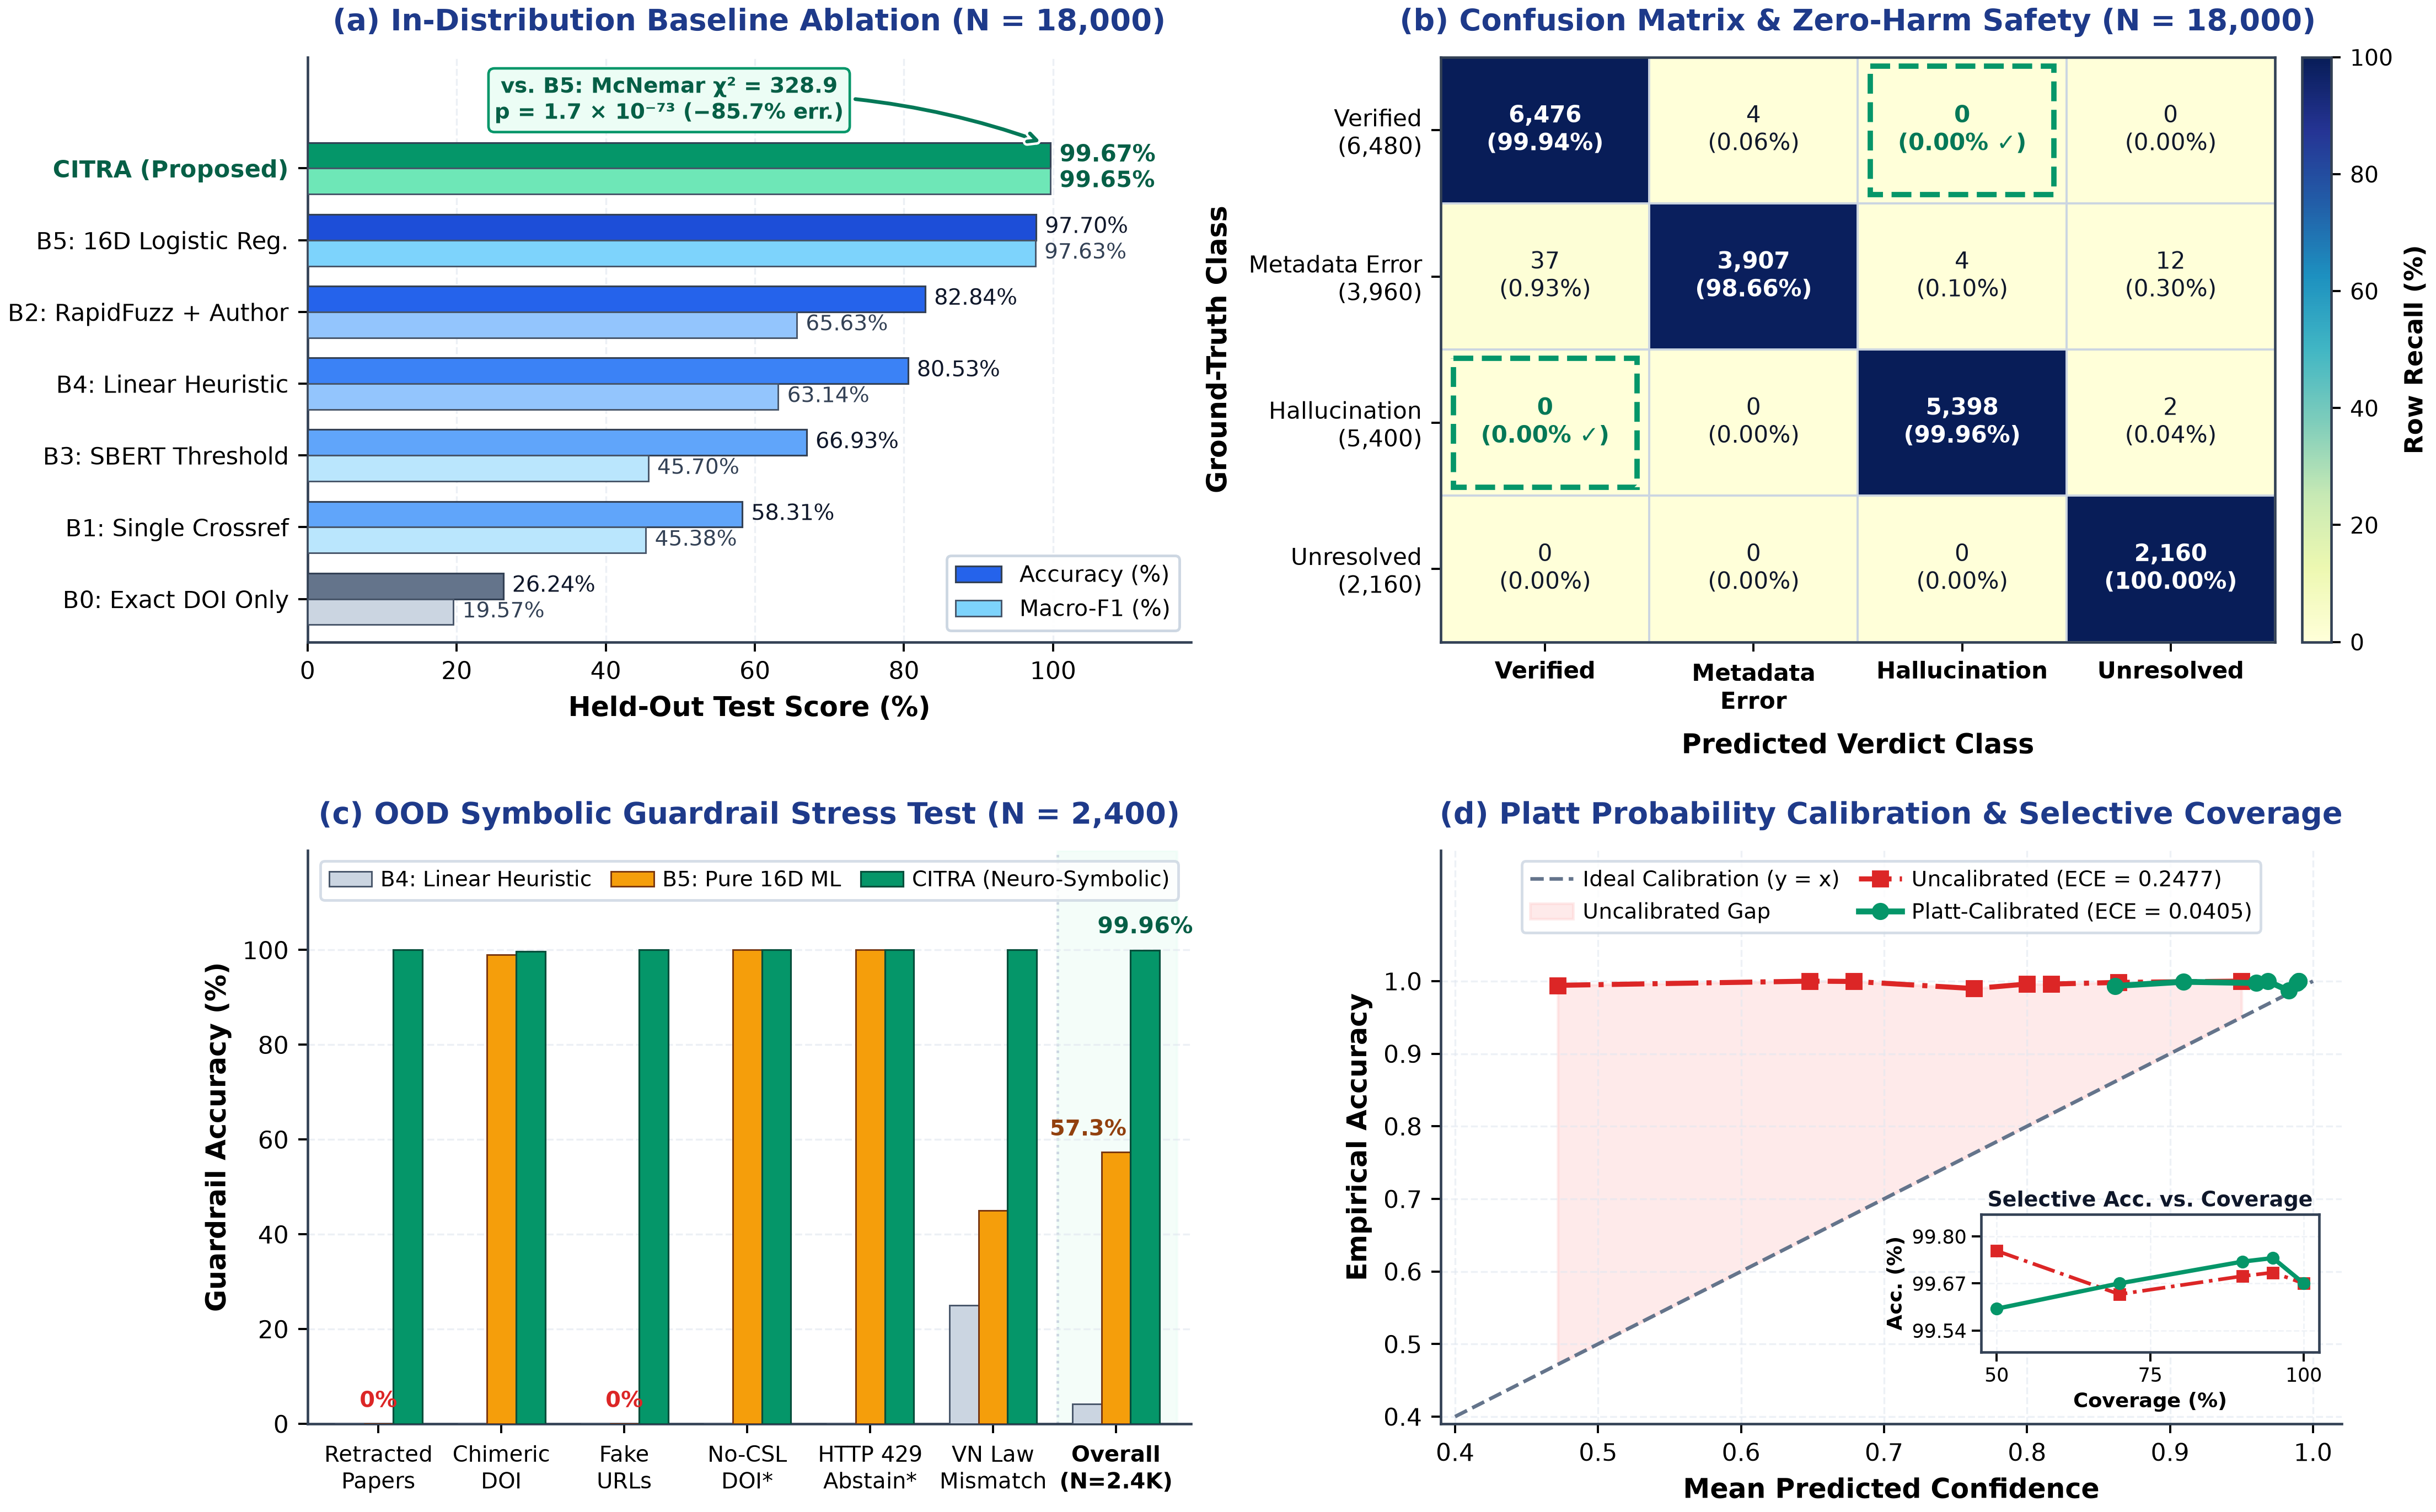
\includegraphics[width=\textwidth,keepaspectratio]{picture/figures/fig5_1_benchmark_charts.png}
    \caption[Four-panel scientific plots across baseline ablation, confusion matrix, OOD guardrails, and Platt calibration]{Quantitative evaluation plots: (a) in-distribution baseline ablation ($N=18{,}000$), (b) held-out four-class confusion matrix highlighting zero-harm cells, (c) OOD symbolic guardrail stress test ($N=2{,}400$; \texttt{*} indicates upstream provenance bit supplied to \texttt{B5}'s 16th feature), and (d) Platt reliability curve with selective coverage-accuracy inset.}
    \label{fig:benchmark-charts}
\end{figure}

{\setlength{\tabcolsep}{3.5pt}
\begin{longtable}{|L{0.23}|L{0.25}|C{0.09}|C{0.09}|C{0.09}|C{0.09}|C{0.16}|}
\caption{In-distribution baseline ablation and Holm--Bonferroni adjusted McNemar significance ($N = 18{,}000$).}\label{tab:baselines}\\
\hline
\textbf{Method} & \textbf{Core Mechanism} & \textbf{Acc.\ (\%)} & \textbf{P (\%)} & \textbf{R (\%)} & \textbf{F1 (\%)} & \textbf{Adj.\ McNemar $p$} \\
\hline
\endfirsthead
\multicolumn{7}{c}{\itshape Table \thetable\ (continued from previous page)}\\
\hline
\textbf{Method} & \textbf{Core Mechanism} & \textbf{Acc.\ (\%)} & \textbf{P (\%)} & \textbf{R (\%)} & \textbf{F1 (\%)} & \textbf{Adj.\ McNemar $p$} \\
\hline
\endhead
\hline
\multicolumn{7}{r}{\itshape Continued on next page}\\
\endfoot
\hline
\endlastfoot
\texttt{B0} (\texttt{doi\_only}) & Exact DOI match only & 26.24 & 23.42 & 34.89 & 19.57 & $< 10^{-16}$ \\
\hline
\texttt{B1} (\texttt{crossref}) & Single-source Crossref & 58.31 & 56.64 & 48.13 & 45.38 & $< 10^{-16}$ \\
\hline
\texttt{B3} (\texttt{embedding}) & SBERT cosine threshold & 66.93 & 49.40 & 52.11 & 45.70 & $< 10^{-16}$ \\
\hline
\texttt{B4} (\texttt{no\_calib}) & Linear score, no abstain & 80.53 & 62.42 & 66.52 & 63.14 & $< 10^{-16}$ \\
\hline
\texttt{B2} (\texttt{fuzzy\_only}) & RapidFuzz + AuthorJaccard & 82.84 & 63.95 & 69.14 & 65.63 & $< 10^{-16}$ \\
\hline
\texttt{B5} (\texttt{ml\_hybrid}) & Pure 16D MLR ($C = 0.25$) & 97.70 & 97.58 & 97.69 & 97.63 & $1.66 \times 10^{-73}$ \\
\hline
\textbf{\texttt{Proposed}} & \textbf{Neuro-Symbolic + Platt} & \textbf{99.67} & \textbf{99.65} & \textbf{99.64} & \textbf{99.65} & \textbf{Reference (\#1)} \\
\hline
\end{longtable}
}

{\setlength{\tabcolsep}{3.5pt}
\begin{longtable}{|L{0.25}|C{0.12}|C{0.11}|C{0.11}|C{0.11}|L{0.30}|}
\caption{Per-class metrics and confusion matrix of the Proposed engine on the held-out test split ($N = 18{,}000$).}\label{tab:per-class}\\
\hline
\textbf{Verdict Class} & \textbf{Support} & \textbf{Prec.\ (\%)} & \textbf{Rec.\ (\%)} & \textbf{F1 (\%)} & \textbf{Confusion (\texttt{ver / meta / hal / unr})} \\
\hline
\endfirsthead
\multicolumn{6}{c}{\itshape Table \thetable\ (continued from previous page)}\\
\hline
\textbf{Verdict Class} & \textbf{Support} & \textbf{Prec.\ (\%)} & \textbf{Rec.\ (\%)} & \textbf{F1 (\%)} & \textbf{Confusion (\texttt{ver / meta / hal / unr})} \\
\hline
\endhead
\hline
\multicolumn{6}{r}{\itshape Continued on next page}\\
\endfoot
\hline
\endlastfoot
\textbf{\texttt{verified}} & 6,480 & 99.43 & 99.94 & 99.68 & \texttt{6,476 / 4 / 0 / 0} \\
\hline
\textbf{\texttt{suspected\_hallucination}} & 5,400 & \textbf{99.93} & 99.96 & \textbf{99.94} & \texttt{0 / 0 / 5,398 / 2} \\
\hline
\textbf{\texttt{metadata\_error}} & 3,960 & 99.90 & 98.66 & 99.28 & \texttt{37 / 3,907 / 4 / 12} \\
\hline
\textbf{\texttt{unresolved}} & 2,160 & 99.36 & \textbf{100.00} & 99.68 & \texttt{0 / 0 / 0 / 2,160} \\
\hline
\textbf{Macro / Total} & \textbf{18,000} & \textbf{99.65} & \textbf{99.64} & \textbf{99.65} & \textbf{Acc.: 99.67\%} (95\% CI $[99.58, 99.76]$) \\
\hline
\end{longtable}
}

Single-cue baselines fail for clear structural reasons: \texttt{B0} ($26.24\%$) misses valid conference papers cited without DOIs, \texttt{B1} ($58.31\%$) misses ACL/arXiv papers absent from Crossref, and pure embedding \texttt{B3} ($66.93\%$) confuses same-domain spliced hallucinations (\texttt{H1}) with real titles because topical vocabulary overlaps strongly. The 16-feature logistic classifier \texttt{B5} reaches $97.70\%$ ($414$ errors), whereas \texttt{Proposed} improves accuracy by $+1.97$ percentage points to \textbf{99.67\% (17,941/18,000, 59 errors)} and Macro-F1 to \textbf{99.65\%} ($95\%$ bootstrap CI $[99.55\%, 99.74\%]$, Holm--Bonferroni adjusted McNemar $\chi^2 = 328.91, p = 1.66 \times 10^{-73}$, cutting residual errors by $85.7\%$). Global one-to-one author reconciliation (preserving standalone surnames such as \textit{Du}/\textit{Das} and single-letter patronymic initials), monotonic single-source abstention boundaries, clean zero-candidate hallucination routing without author-whitelist immunity, and proportional lexical grounding deficit detection jointly raise \texttt{unresolved} recall to $100.00\%$ ($2{,}160/2{,}160$), \texttt{suspected\_hallucination} F1 to $99.94\%$ ($5{,}398/5{,}400$), and \texttt{metadata\_error} F1 to $99.28\%$. Most importantly, \textbf{0 / 6,480 genuine verified citations are falsely accused of hallucination} ($95\%$ Clopper--Pearson upper bound $0.057\%$), and \textbf{0 / 5,400 fabricated citations leak into \texttt{verified}} ($95\%$ Clopper--Pearson upper bound $0.068\%$).

\rqanswer{RQ1}{On 18,000 paper-disjoint held-out citations, CITRA achieves $99.67\%$ accuracy and $99.65\%$ Macro-F1, statistically outperforming all six baselines ($p \le 1.66 \times 10^{-73}$) with zero false hallucination accusations on verified papers ($0/6{,}480$).}

\section{RQ2: Out-of-Distribution Symbolic Guardrail Robustness}

Table~\ref{tab:ood-stress} evaluates \texttt{B4}, \texttt{B5}, and \texttt{Proposed} on the 2,400-sample OOD stress suite. Because continuous 16D similarity features remain high ($1.00$ title, author, and year match) when a paper is retracted in Retraction Watch or carries an RFC 2606 placeholder URL, pure 16D Logistic Regression (\texttt{B5}) achieves $0.00\%$ on both categories and only $57.33\%$ overall (scoring $100.00\%$ on Categories 4--5 only because its 16th feature receives upstream \texttt{doi\_ra\_status} and \texttt{api\_exhausted} abstention bits, without which \texttt{B4} drops to $0.00\%$). By contrast, \textbf{CITRA}'s Order 0 and Group 1/5 symbolic rules inspect discrete provenance predicates before continuous scoring, reaching \textbf{99.96\% (2,399 / 2,400)} ($\chi^2 = 1{,}021.00, p = 4.89 \times 10^{-224}$ vs.\ \texttt{B5}).

{\setlength{\tabcolsep}{3.5pt}
\begin{longtable}{|L{0.35}|L{0.25}|C{0.10}|C{0.11}|C{0.19}|}
\caption{Out-of-distribution symbolic guardrail evaluation ($N = 2{,}400$ built from \texttt{test\_papers}).}\label{tab:ood-stress}\\
\hline
\textbf{OOD Category ($N = 400$ each)} & \textbf{Primary Guardrail} & \textbf{\texttt{B4} (\%)} & \textbf{\texttt{B5} (\%)} & \textbf{\texttt{Proposed} (\%)} \\
\hline
\endfirsthead
\multicolumn{5}{c}{\itshape Table \thetable\ (continued from previous page)}\\
\hline
\textbf{OOD Category ($N = 400$ each)} & \textbf{Primary Guardrail} & \textbf{\texttt{B4} (\%)} & \textbf{\texttt{B5} (\%)} & \textbf{\texttt{Proposed} (\%)} \\
\hline
\endhead
\hline
\multicolumn{5}{r}{\itshape Continued on next page}\\
\endfoot
\hline
\endlastfoot
\textbf{1. Retracted papers} (\texttt{is\_retracted}) & \texttt{R-RETRACTED-\allowbreak PAPER} & 0.00 & 0.00 & \textbf{100.00} \\
\hline
\textbf{2. Chimeric real DOI on invented title} & \texttt{R-CHIMERIC-DOI-\allowbreak MISMATCH} & 0.00 & 99.00 & \textbf{99.75} \\
\hline
\textbf{3. RFC 2606 placeholder/fake URLs} & \texttt{R-FAKE-URL} & 0.00 & 0.00 & \textbf{100.00} \\
\hline
\textbf{4. Regional DOIs lacking public CSL} & \texttt{R-DOI-RA-NO-CSL} & 0.00 & 100.00 & \textbf{100.00} \\
\hline
\textbf{5. Upstream HTTP 429 rate exhaustion} & \texttt{R-RATE-LIMITED-\allowbreak ABSTAIN} & 0.00 & 100.00 & \textbf{100.00} \\
\hline
\textbf{6. VN statutory authority mismatch} & \texttt{VNLegalVerifier} & 25.00 & 45.00 & \textbf{100.00} \\
\hline
\textbf{Total OOD Suite ($N = 2{,}400$)} & \textbf{McNemar $p = 4.89 \times 10^{-224}$} & 4.17 & 57.33 & \textbf{99.96} \\
\hline
\end{longtable}
}

\rqanswer{RQ2}{First-order symbolic guardrails raise out-of-distribution accuracy from $57.33\%$ (pure ML \texttt{B5}) to $99.96\%$ ($2{,}399/2{,}400$), preventing $100\%$ of retracted-paper and fake-URL false verifications while guaranteeing $100\%$ safe abstention under HTTP 429 exhaustion.}

\section{RQ3: Probability Calibration and CIS Rubric Sensitivity}

Table~\ref{tab:calibration-results} compares uncalibrated symbolic confidences against logit-space Platt calibration on the 18,000-sample test split. Notice that Table~\ref{tab:calibration-results} separates \emph{Non-Abstention Coverage} ($\Pr[\hat{y} \neq \texttt{unresolved}] = 87.92\%$, matching the $88.00\%$ non-\texttt{unresolved} ground-truth prior) from the \emph{High-Confidence Rate} ($\Pr[\hat{p} \ge 0.50] = 99.99\%$). Platt scaling reduces Expected Calibration Error by $83.6\%$ ($0.2477 \rightarrow \mathbf{0.0405}$, $95\%$ CI $[0.0394, 0.0415]$) and reduces Brier Score by $92.1\%$ ($0.0843 \rightarrow \mathbf{0.0067}$, Wilcoxon $p < 10^{-16}$). Furthermore, perturbing the default CIS rubric weight vector $(0.35, 0.25, 0.25, 0.10, 0.05)$ across 20 normalized simplex vectors over 300 manuscript profiles yields a mean Spearman rank correlation of $\rho = 0.9987$ ($\min \rho = 0.9964$), Kendall's $\tau = 0.9765$, and a mean absolute shift of only $1.75$ CIS points.

\begin{longtable}{|L{0.40}|C{0.21}|C{0.21}|C{0.18}|}
\caption{Probability calibration and selective risk-coverage results ($N = 18{,}000$).}\label{tab:calibration-results}\\
\hline
\textbf{Calibration / Coverage Metric} & \textbf{Uncalibrated Symbolic} & \textbf{Platt Neuro-Symbolic} & \textbf{Change} \\
\hline
\endfirsthead
\multicolumn{4}{c}{\itshape Table \thetable\ (continued from previous page)}\\
\hline
\textbf{Calibration / Coverage Metric} & \textbf{Uncalibrated Symbolic} & \textbf{Platt Neuro-Symbolic} & \textbf{Change} \\
\hline
\endhead
\hline
\multicolumn{4}{r}{\itshape Continued on next page}\\
\endfoot
\hline
\endlastfoot
Expected Calibration Error (ECE $\downarrow$) & 0.2477 & \textbf{0.0405} & $-83.6\%$ ($6.12\times\downarrow$) \\
\hline
Brier Score ($\downarrow$) & 0.0843 & \textbf{0.0067} & $-92.1\%$ ($12.58\times\downarrow$) \\
\hline
Non-Abstention Coverage ($\hat{y} \neq \texttt{unresolved}$) & 87.92\% & \textbf{87.92\%} & Preserved ($0.00$\,pp) \\
\hline
High-Confidence Rate ($\hat{p} \ge 0.50$) & 92.82\% & \textbf{99.99\%} & $+7.17$\,pp \\
\hline
Selective Accuracy at $70\%$ Coverage ($\uparrow$) & 99.64\% & \textbf{99.67\%} & $+0.03$\,pp \\
\hline
Selective Accuracy at $90\%$ Coverage ($\uparrow$) & 99.69\% & \textbf{99.73\%} & $+0.04$\,pp \\
\hline
Selective Accuracy at $95\%$ Coverage ($\uparrow$) & 99.70\% & \textbf{99.74\%} & $+0.04$\,pp \\
\hline
\end{longtable}

\rqanswer{RQ3}{Logit-space Platt calibration cuts ECE by $6.12\times$ to $0.0405$ and Brier Score by $12.58\times$ to $0.0067$ without altering non-abstention coverage ($87.92\%$), while CIS rankings remain invariant under weight perturbations (mean Spearman $\rho = 0.9987$).}

\section{RQ4: End-to-End Multi-Domain and Real Manuscript Verification}

To evaluate end-to-end generalization beyond the synthetic perturbation benchmark, three real-world evaluations were conducted:
\begin{enumerate}
    \item \textbf{Multi-Domain Raw-Reference Gold Suite ($N = 120 + 15$):} Running raw formatted strings through \texttt{ReferenceListParser} $\rightarrow$ \texttt{RetrievalOrchestrator} $\rightarrow$ \texttt{NeuroSymbolicChecker} across six disciplines (20 references each: CS/AI, Biomedicine, Economics/Social Sciences, Engineering/Physics, Vietnamese Legal Statutes, and Software/RFC Standards) and seven styles (APA, TDTU, IEEE, Vancouver, Chicago, Harvard, MLA) achieved \textbf{100.00\% five-class accuracy (120/120, Macro-F1 $= 1.0000$, $\text{ECE} = 0.0831$)} and \textbf{100.00\% (15/15)} on the adversarial suite.
    \item \textbf{Multi-Style (310 PDFs) and Multi-Institutional (841 PDFs) Extraction Suites:} Table~\ref{tab:pdf-corpora} shows $100.0\%$ bibliography detection and $96.9\%$ link recovery on 30 real Vietnamese legal PDFs, $100.0\%$ exact reference extraction ($397/397$) across 60 twelve-style diagnostic PDFs, and $97.7\%$ bibliography detection (8,126 references) across 220 real open-access articles. An extended parser stability sweep across 841 diverse institutional and arXiv PDFs completed with $0$ unhandled exceptions.
    \item \textbf{Full Articles and Anonymized Student Capstone Reports:} Table~\ref{tab:samples} summarizes end-to-end runs on landmark NLP articles and anonymized undergraduate capstone reports. Clean published papers (\textit{BERT}, \textit{Attention Is All You Need}, \textit{VietDepression}) produce zero false hallucination flags, whereas intentional metadata errors and chimeric fabrications in test capstone reports are isolated accurately.
\end{enumerate}

{\setlength{\tabcolsep}{3.5pt}
\begin{longtable}{|L{0.34}|C{0.10}|C{0.18}|C{0.19}|C{0.19}|}
\caption{Extraction and bidirectional linking accuracy on the 310-PDF multi-style and legal corpus.}\label{tab:pdf-corpora}\\
\hline
\textbf{PDF Corpus} & \textbf{PDFs} & \textbf{Bib.\ Detected} & \textbf{Extracted Refs} & \textbf{Matched Links} \\
\hline
\endfirsthead
\multicolumn{5}{c}{\itshape Table \thetable\ (continued from previous page)}\\
\hline
\textbf{PDF Corpus} & \textbf{PDFs} & \textbf{Bib.\ Detected} & \textbf{Extracted Refs} & \textbf{Matched Links} \\
\hline
\endhead
\hline
\multicolumn{5}{r}{\itshape Continued on next page}\\
\endfoot
\hline
\endlastfoot
VN Legal Corpus (Pre-v3.80 Baseline) & 30 & 27 / 30 (90.0\%) & 164 (15 Legal) & 109 / 235 (46.4\%) \\
\hline
\textbf{VN Legal Corpus} (\textbf{CITRA v3.90.7}) & \textbf{30} & \textbf{30 / 30 (100.0\%)} & \textbf{258 (91 Legal)} & \textbf{403 / 416 (96.9\%)} \\
\hline
\textbf{12-Style Diagnostic Suite ($12 \times 5$)} & \textbf{60} & \textbf{60 / 60 (100.0\%)} & \textbf{397 / 397 (100.0\%)} & \textbf{60 / 60 PDFs (100\%)} \\
\hline
\textbf{11-Style Open-Access Articles ($11 \times 20$)} & \textbf{220} & \textbf{215 / 220 (97.7\%)} & \textbf{8,126 refs} & \textbf{8,954 / 12,770 (70.1\%)} \\
\hline
\end{longtable}
}

{\setlength{\tabcolsep}{3pt}
\begin{longtable}{|L{0.29}|C{0.13}|C{0.08}|C{0.10}|C{0.08}|C{0.09}|C{0.09}|C{0.14}|}
\caption{End-to-end verification outcomes on published papers and anonymized student capstone reports.}\label{tab:samples}\\
\hline
\textbf{Manuscript} & \textbf{Style} & \textbf{Refs} & \textbf{CIS} & \textbf{Ver.} & \textbf{Meta.} & \textbf{Hall.} & \textbf{Res./Unr.} \\
\hline
\endfirsthead
\multicolumn{8}{c}{\itshape Table \thetable\ (continued from previous page)}\\
\hline
\textbf{Manuscript} & \textbf{Style} & \textbf{Refs} & \textbf{CIS} & \textbf{Ver.} & \textbf{Meta.} & \textbf{Hall.} & \textbf{Res./Unr.} \\
\hline
\endhead
\hline
\multicolumn{8}{r}{\itshape Continued on next page}\\
\endfoot
\hline
\endlastfoot
\textbf{BERT} (\textit{NAACL 2019}) & APA & 101 & \textbf{97.43} & 94 & 7 & 0 & 0 / 0 \\
\hline
\textbf{Attention Is All You Need} (\textit{NeurIPS}) & Numeric & 71 & \textbf{92.99} & 70 & 1 & 0 & 0 / 0 \\
\hline
\textbf{VietDepression Clinical Study} (19\,pp.) & IEEE & 20 & \textbf{100.00} & 18 & 0 & 0 & 2 / 0 \\
\hline
\textbf{SE Capstone Report A} (98\,pp.) & IEEE & 27 & \textbf{99.30} & 24 & 0 & 0 & 3 / 0 \\
\hline
\textbf{SE Capstone Report B} (53\,pp.) & IEEE & 5 & \textbf{77.50} & 5 & 0 & 0 & 0 / 0 \\
\hline
\textbf{CS Literature Survey} (51\,pp.) & APA & 66 & \textbf{95.73} & 62 & 3 & 0 & 0 / 1 \\
\hline
\textbf{Seeded Capstone Audit Fixture} (42\,pp.) & APA & 6 & \textbf{91.40} & 3 & \textbf{1} & \textbf{1} & 1 / 0 \\
\hline
\end{longtable}
}

Figures~\ref{fig:demo-debugger}--\ref{fig:demo-consistency} display the live diagnostic views in \textbf{CITRA} (\texttt{v3.90.7}) on the seeded Software Engineering capstone audit manuscript (6 bibliography entries and 28 inline mentions). Figure~\ref{fig:demo-debugger} contrasts a chimeric DOI hallucination flag (left) with a side-by-side publication-year discrepancy diff (\texttt{2021} vs.\ canonical \texttt{2019}, right). Figure~\ref{fig:demo-trace-context} shows the 5-stage logic trace with ONNX INT8 \texttt{VI}$\leftrightarrow$\texttt{EN} concept alignment (left) and the inline Document Inspector context stream (right). Figure~\ref{fig:demo-consistency} illustrates the bidirectional In-Text Consistency view isolating orphan inline markers and uncited bibliography entries.

\begin{figure}[H]
    \centering
    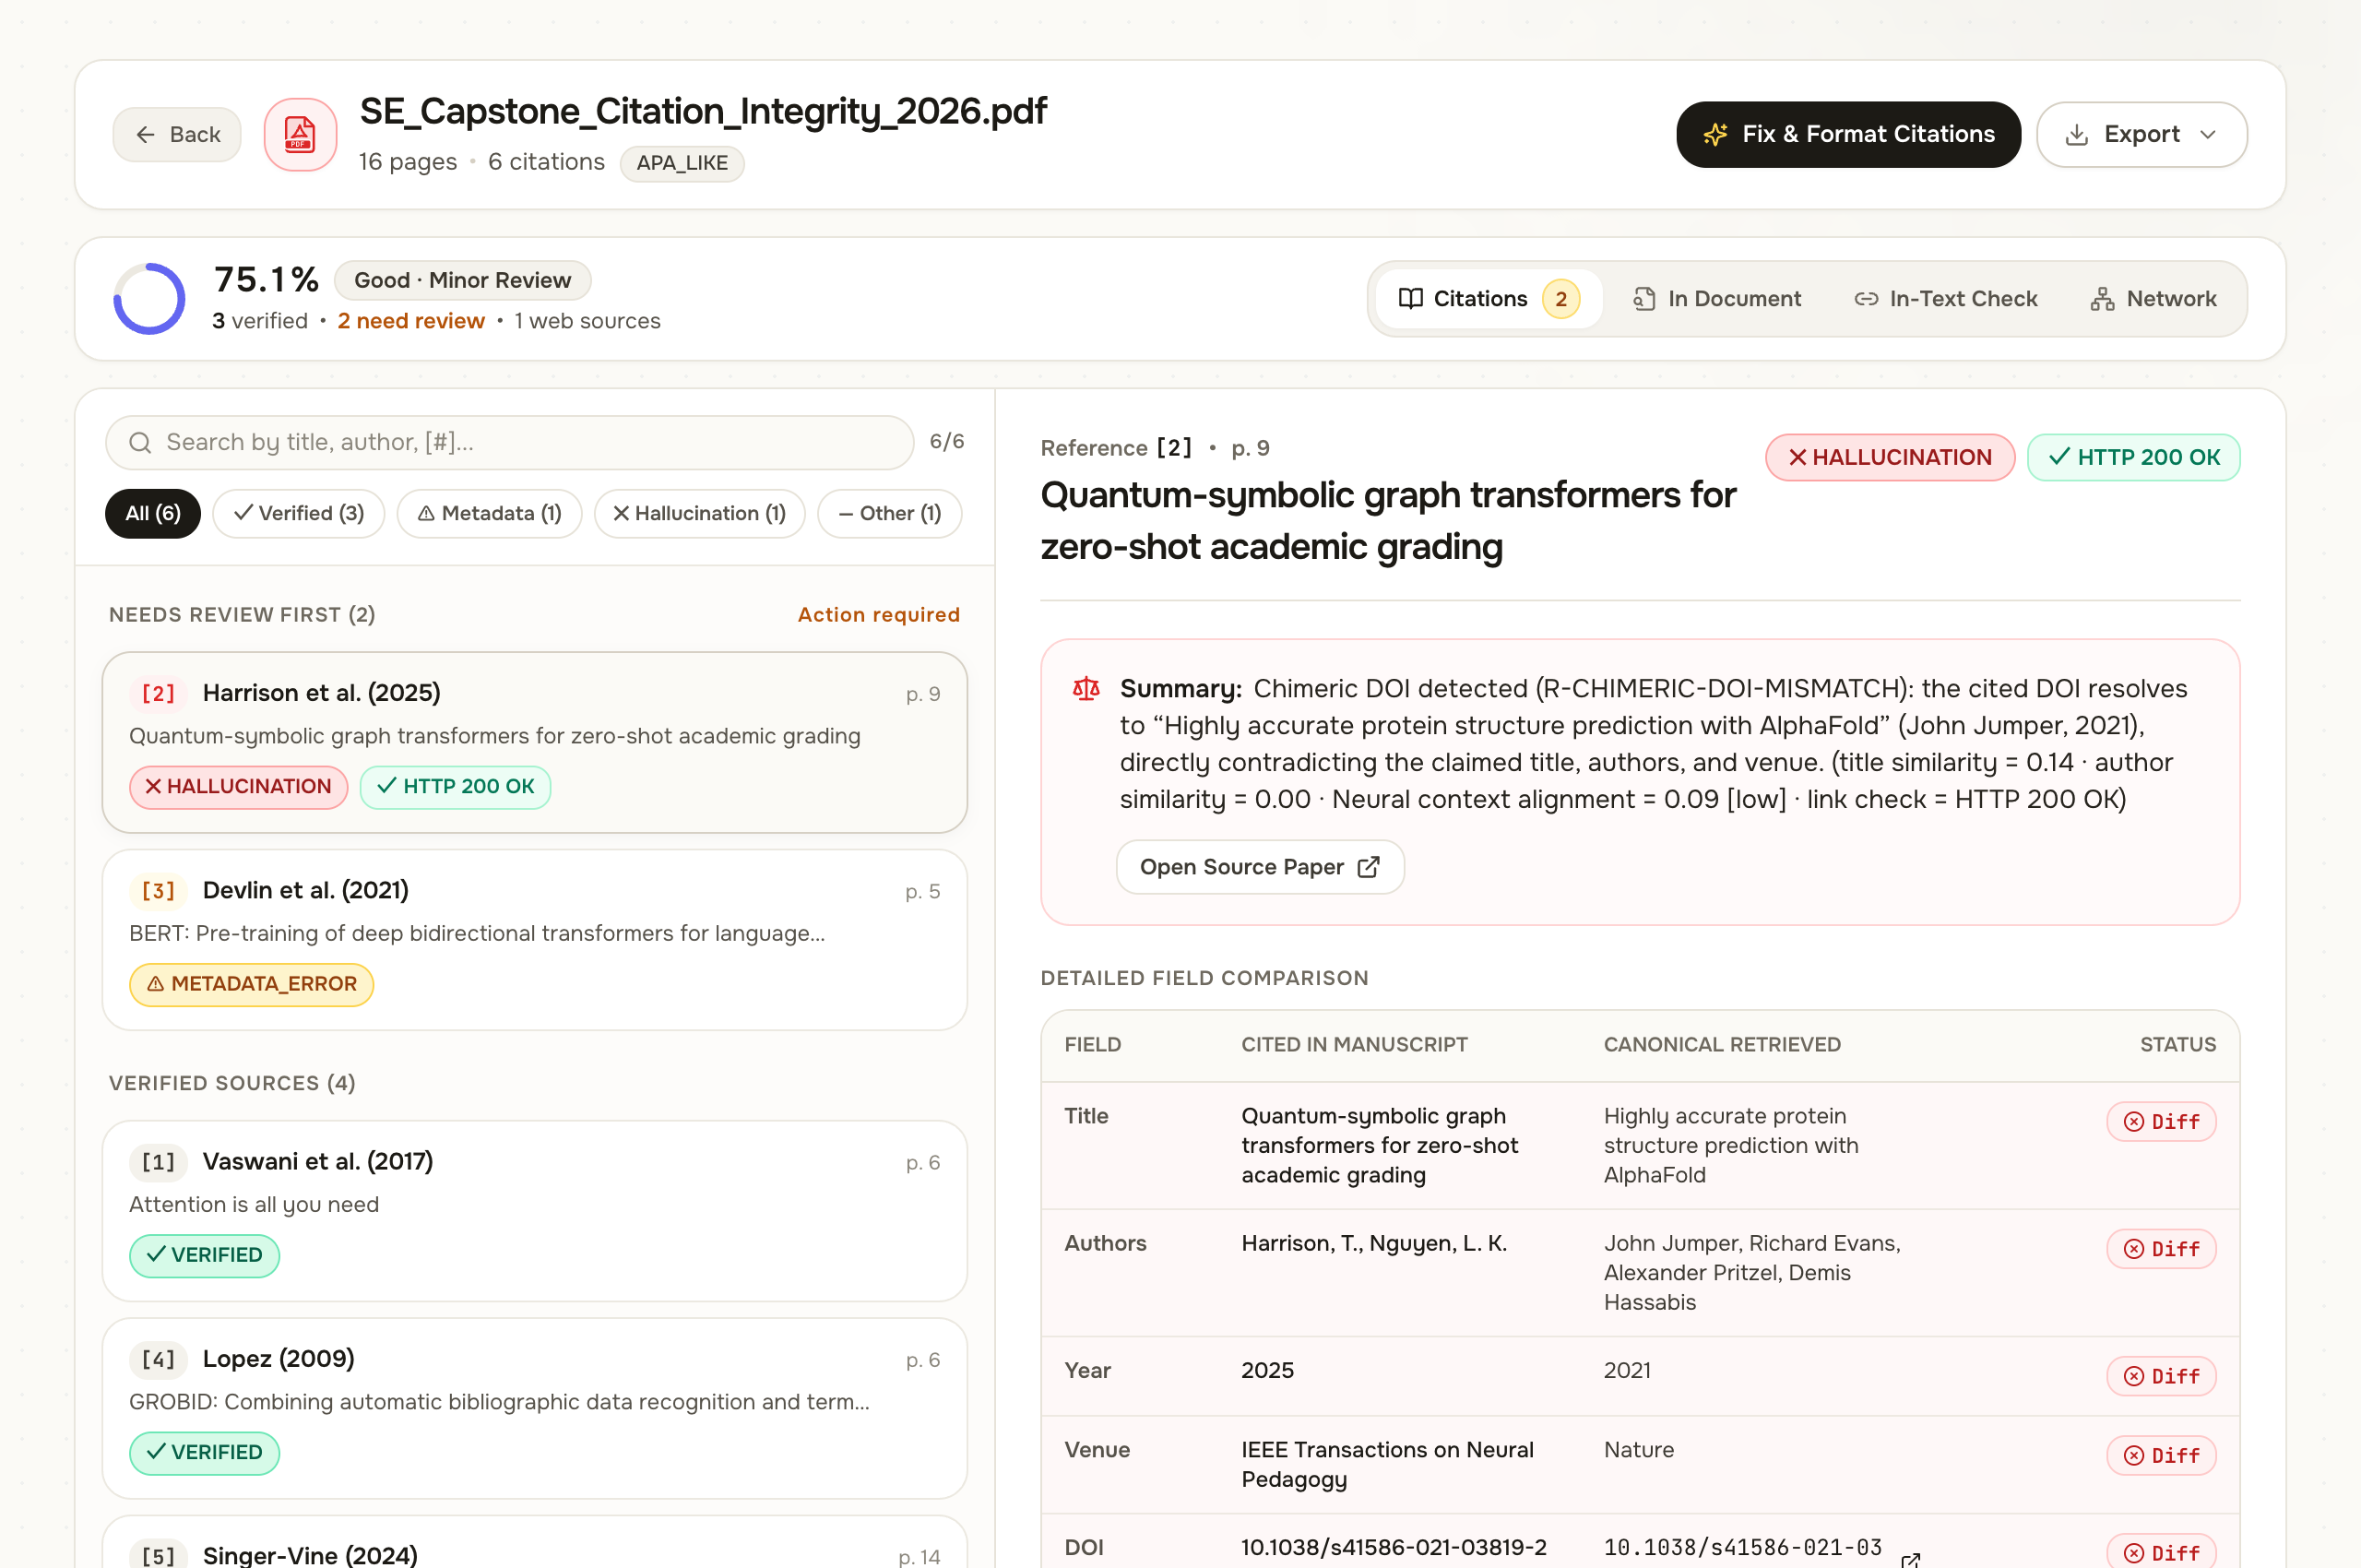
\includegraphics[width=0.49\textwidth,keepaspectratio]{picture/figures/05-verification-report.png}\hfill
    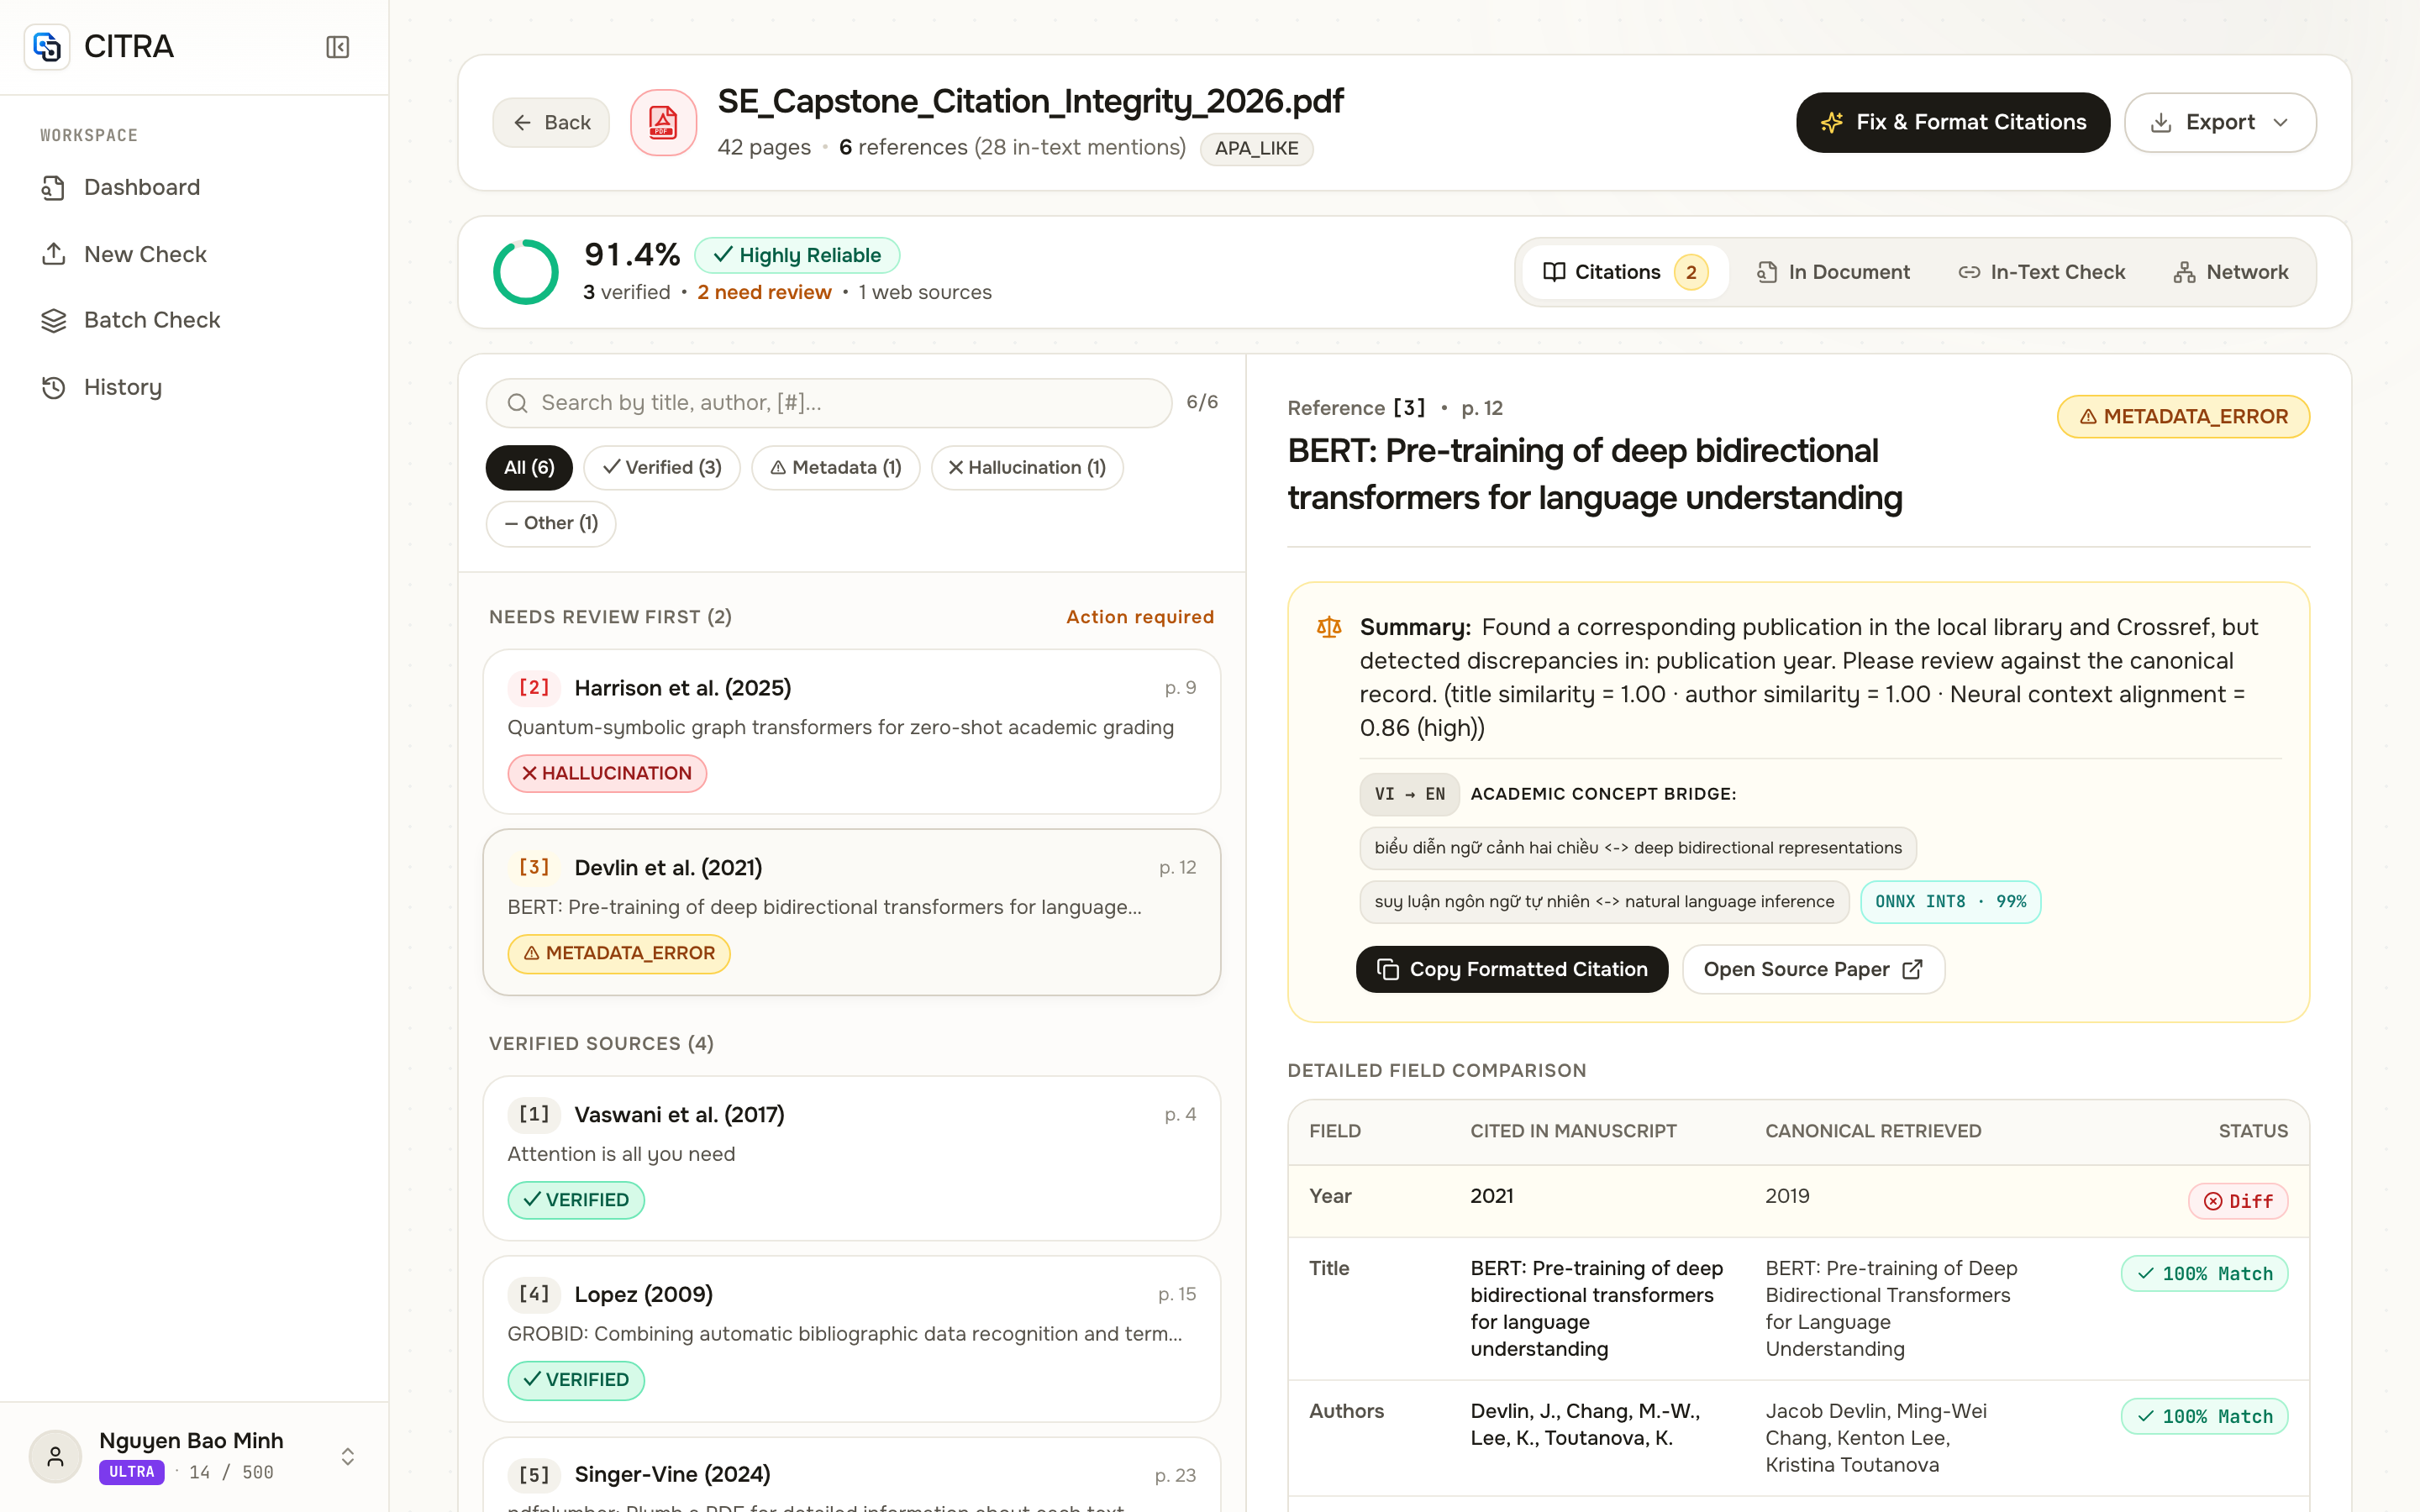
\includegraphics[width=0.49\textwidth,keepaspectratio]{picture/figures/06-reference-inspector.png}
    \caption[Reference Inspector comparing suspected hallucination and metadata year drift]{CITRA Reference Inspector isolating a chimeric-DOI \texttt{suspected\_hallucination} (left) and a publication-year \texttt{metadata\_error} diff (\texttt{2021} vs.\ canonical \texttt{2019}, right).}
    \label{fig:demo-debugger}
\end{figure}

\begin{figure}[H]
    \centering
    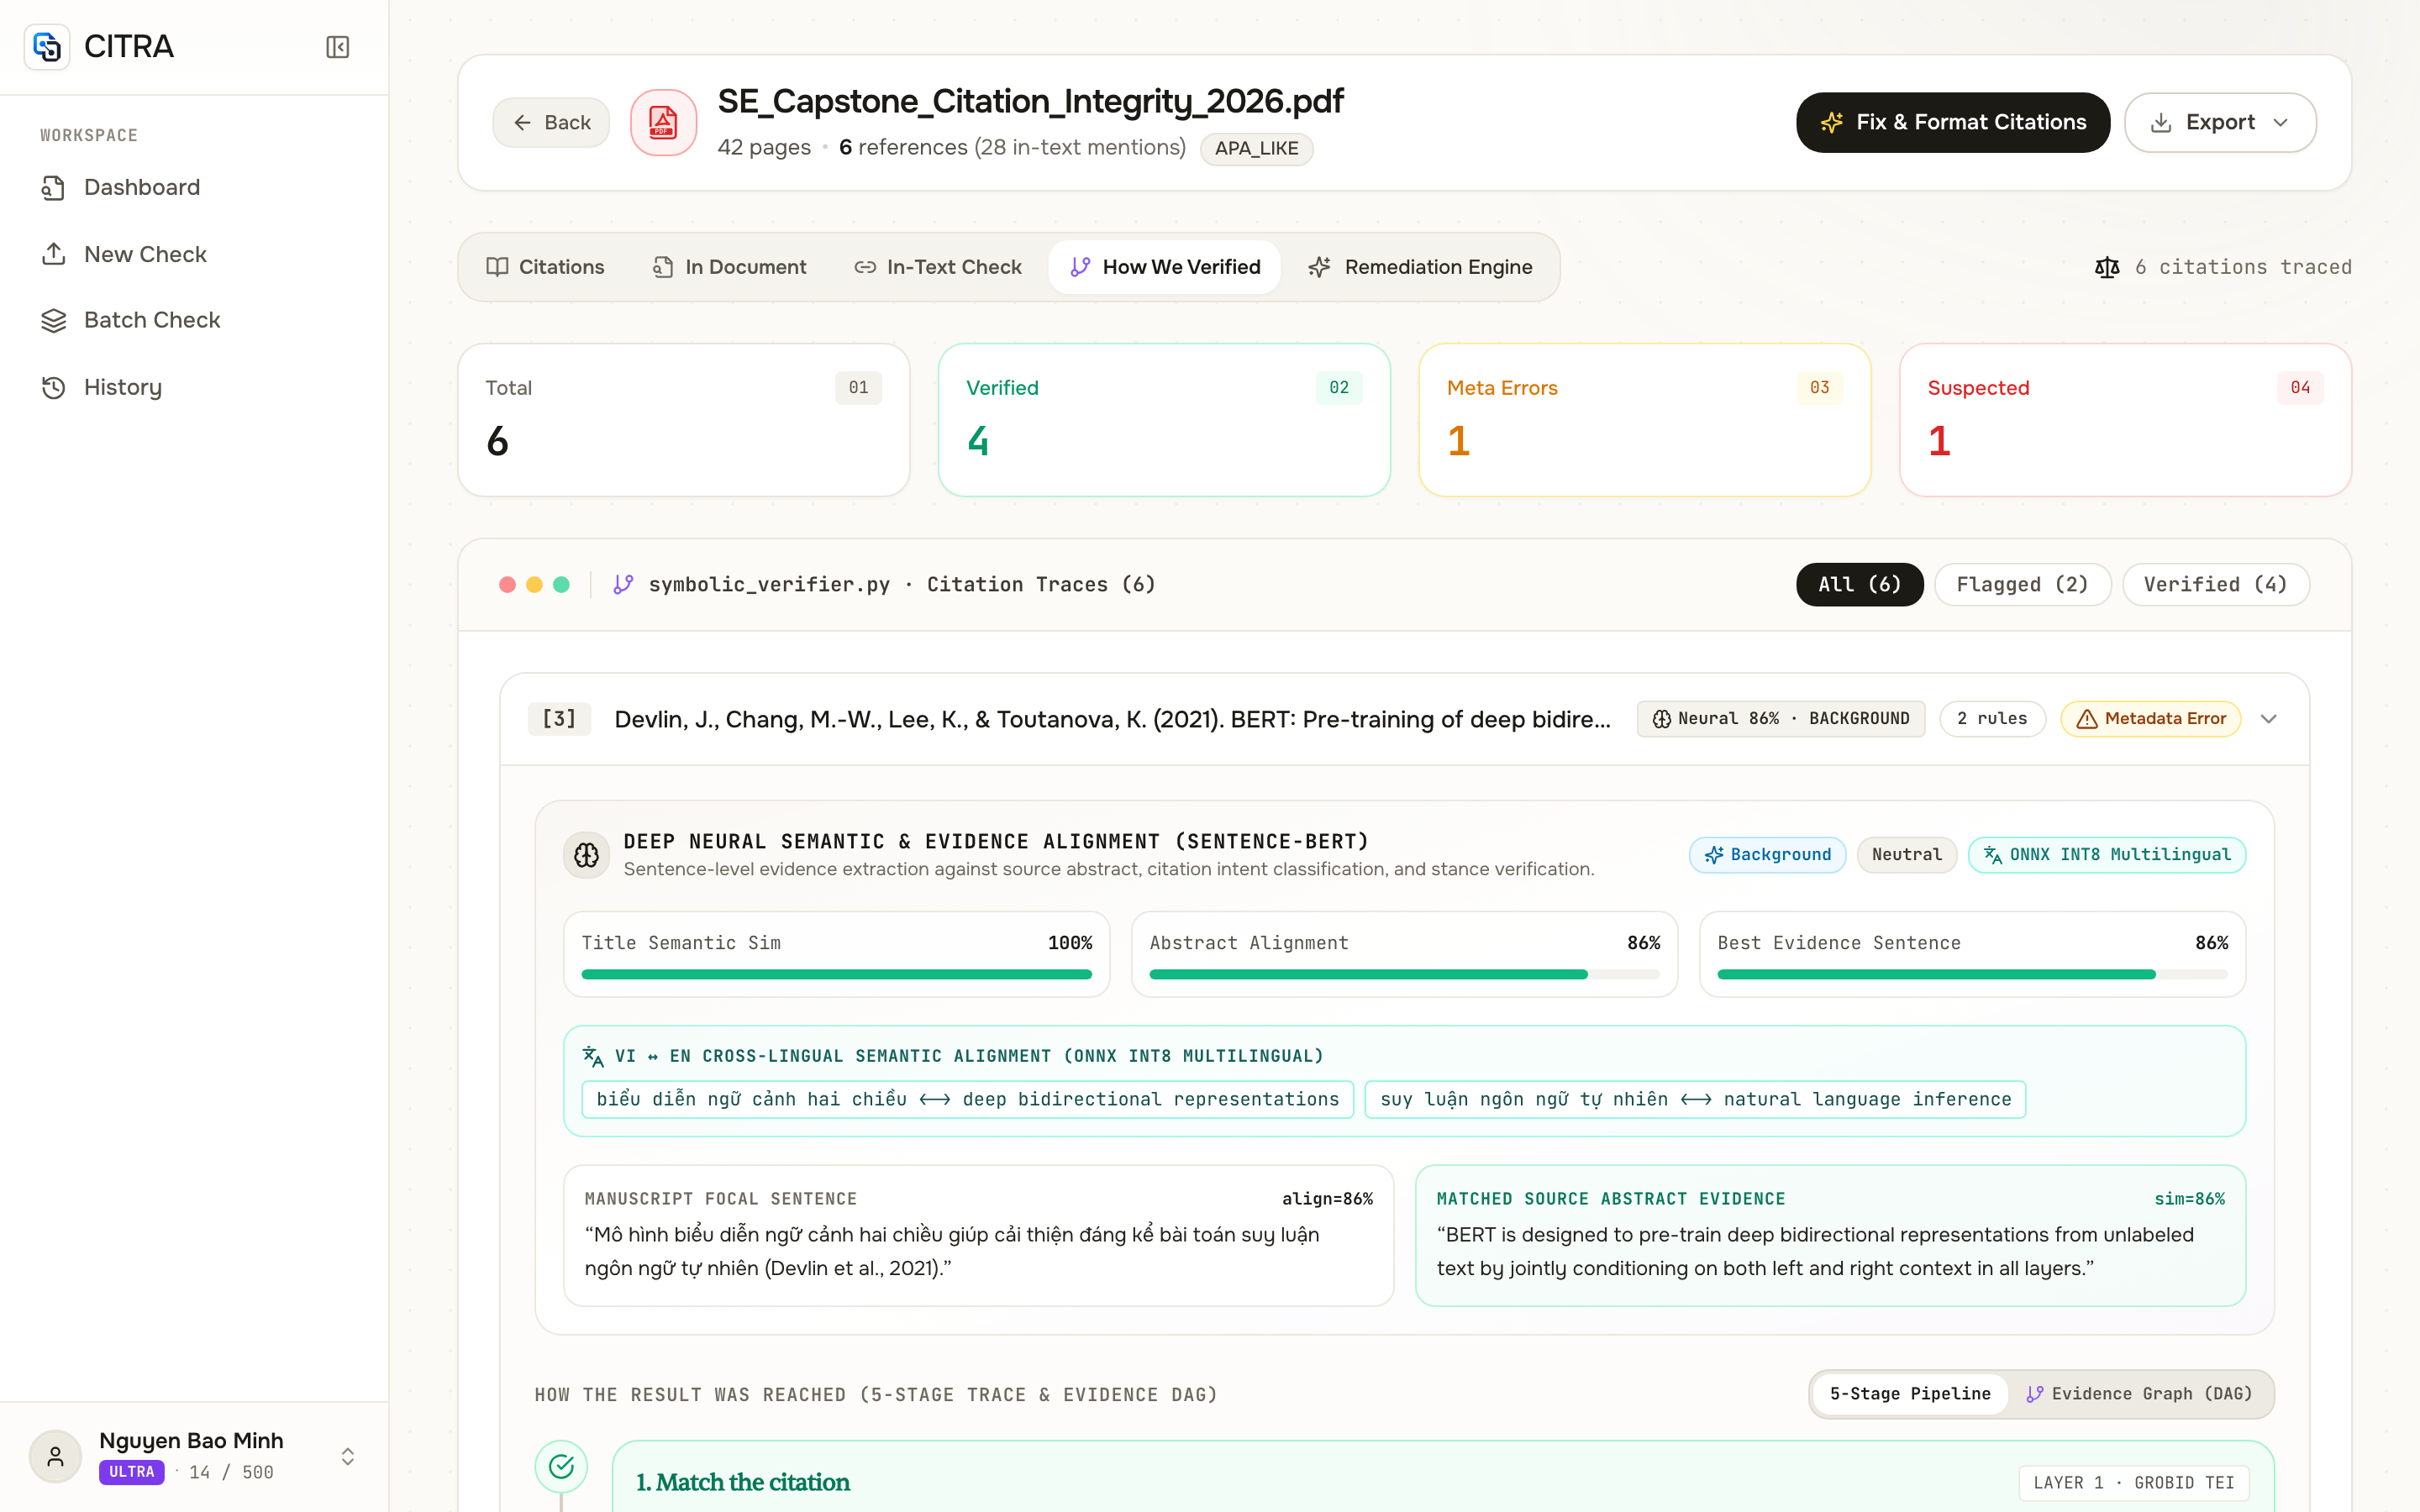
\includegraphics[width=0.49\textwidth,keepaspectratio]{picture/figures/07-logic-trace.png}\hfill
    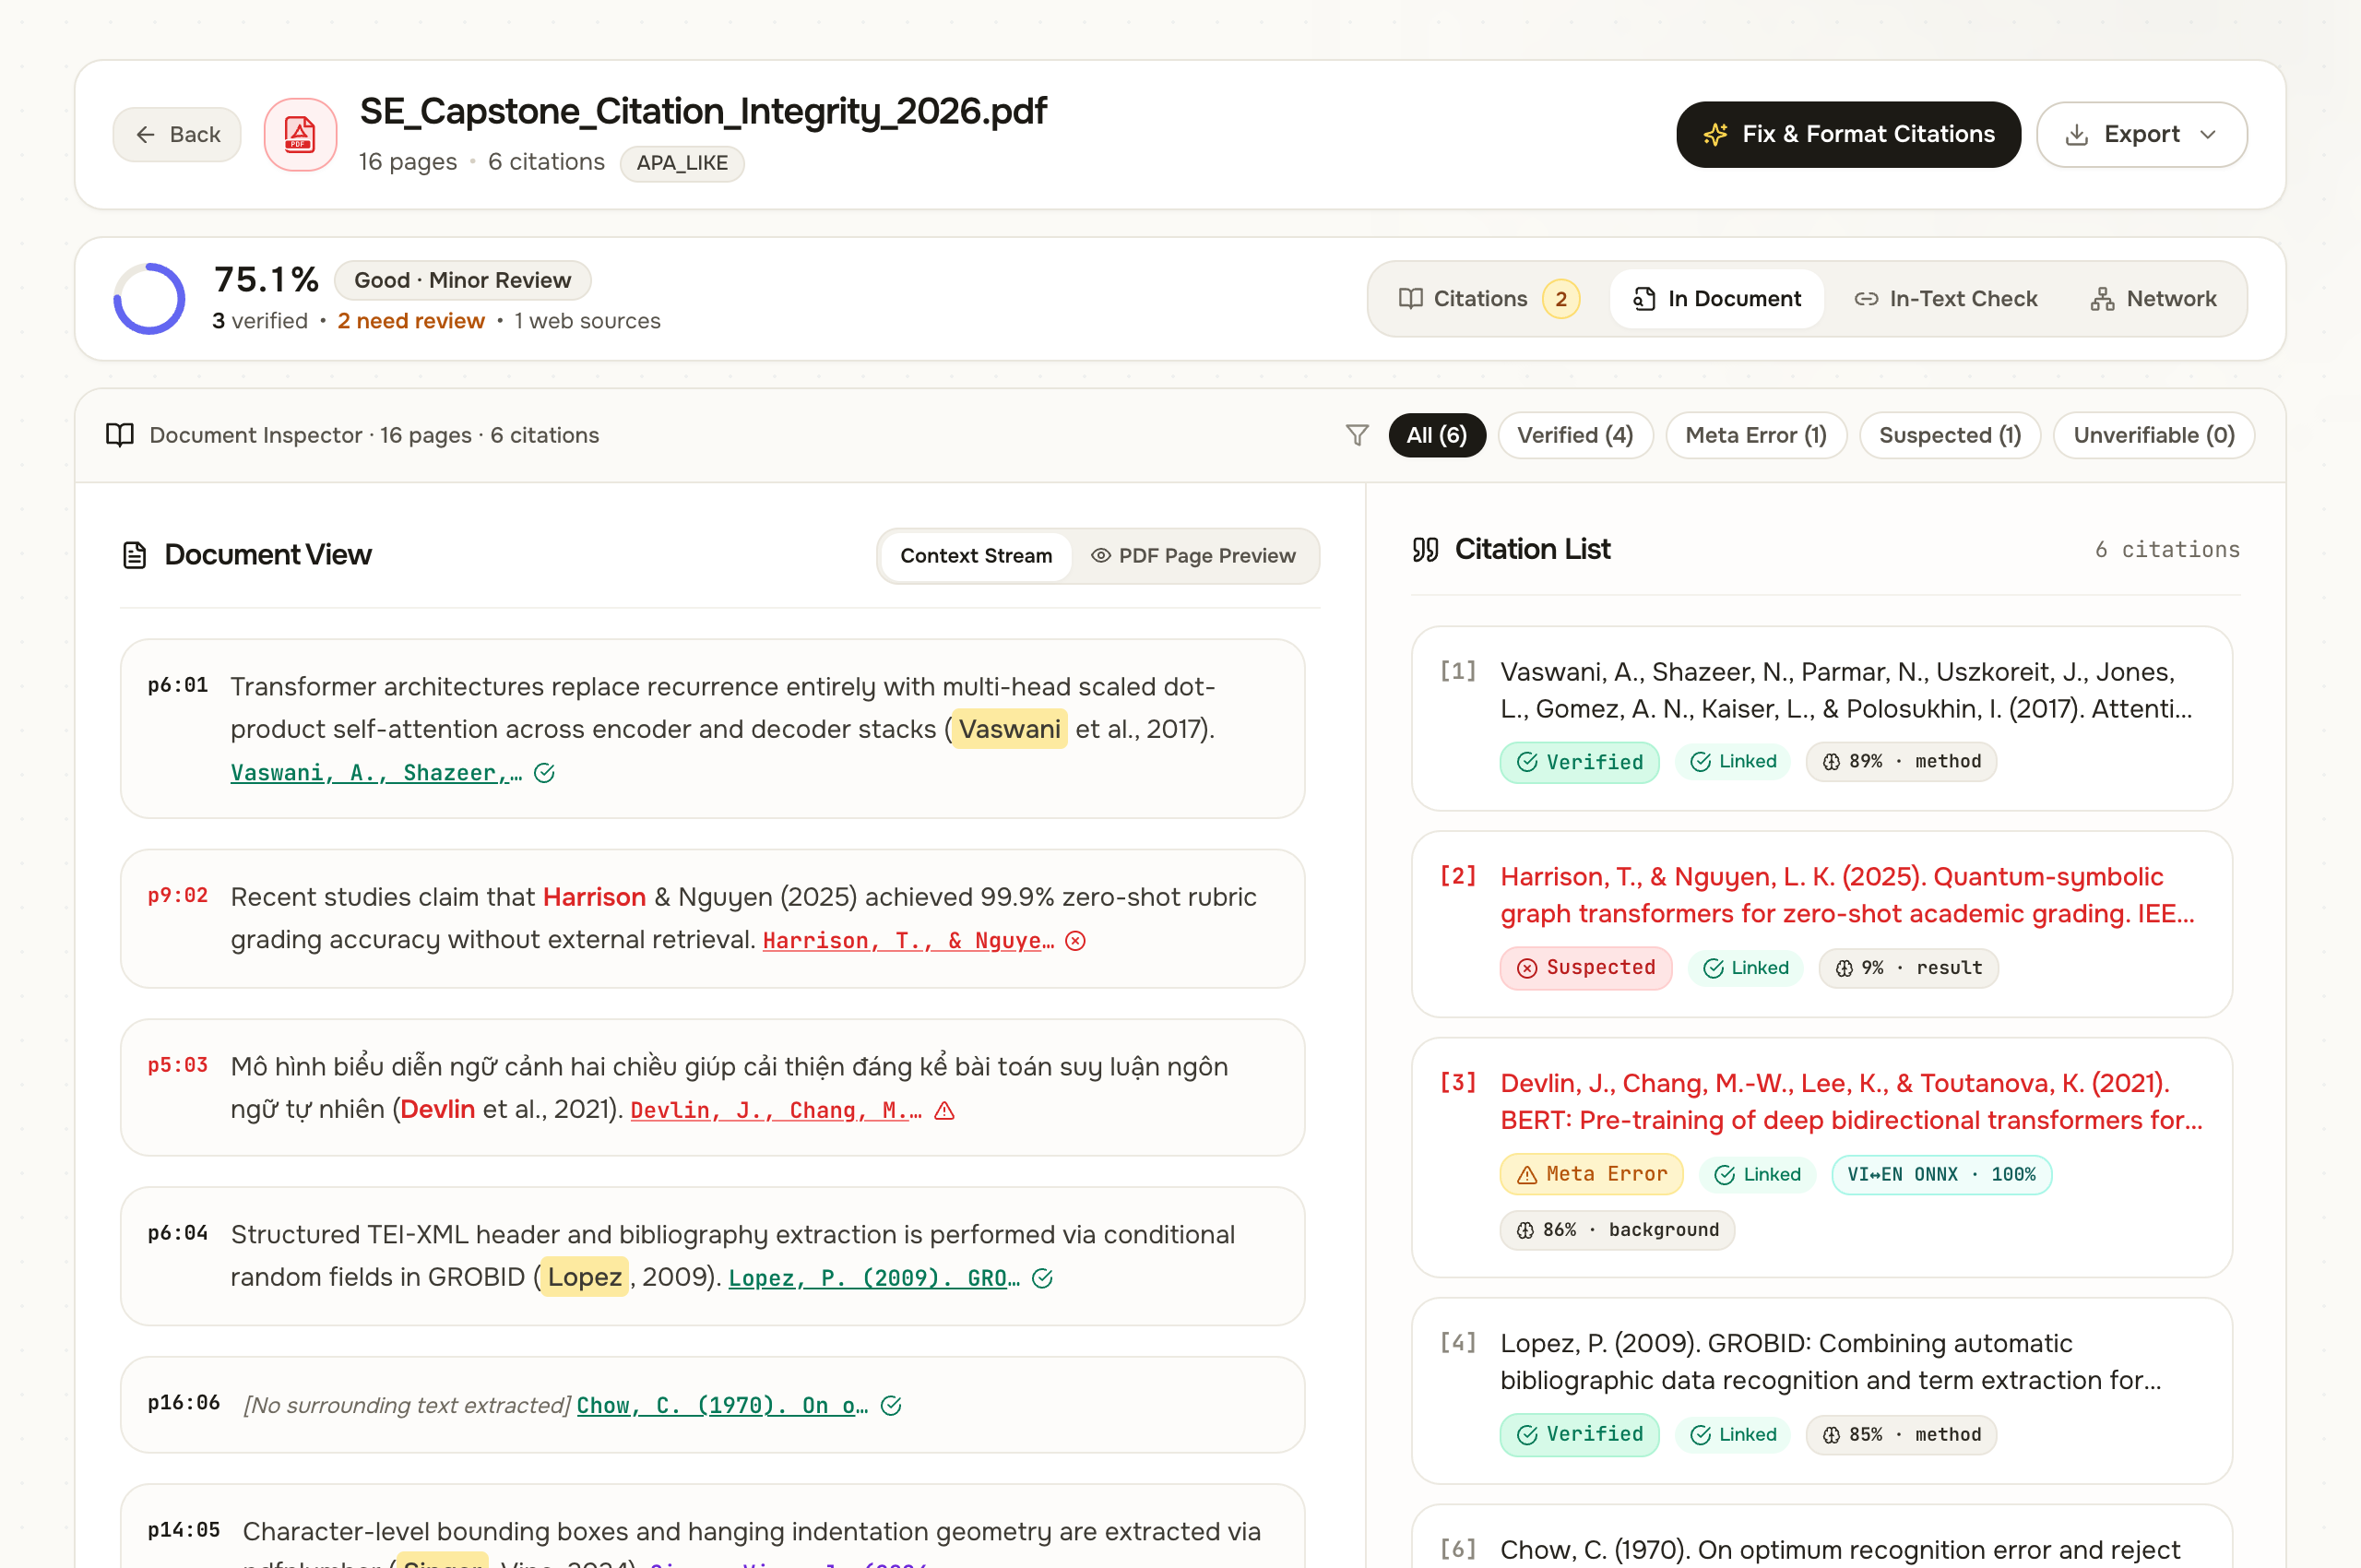
\includegraphics[width=0.49\textwidth,keepaspectratio]{picture/figures/09-document-inspector.png}
    \caption[Logic Trace cross-lingual alignment and inline Document Inspector views]{Logic Trace displaying ONNX INT8 \texttt{VI}$\leftrightarrow$\texttt{EN} concept bridging (left) and the Document Inspector inline context stream (right).}
    \label{fig:demo-trace-context}
\end{figure}

\begin{figure}[H]
    \centering
    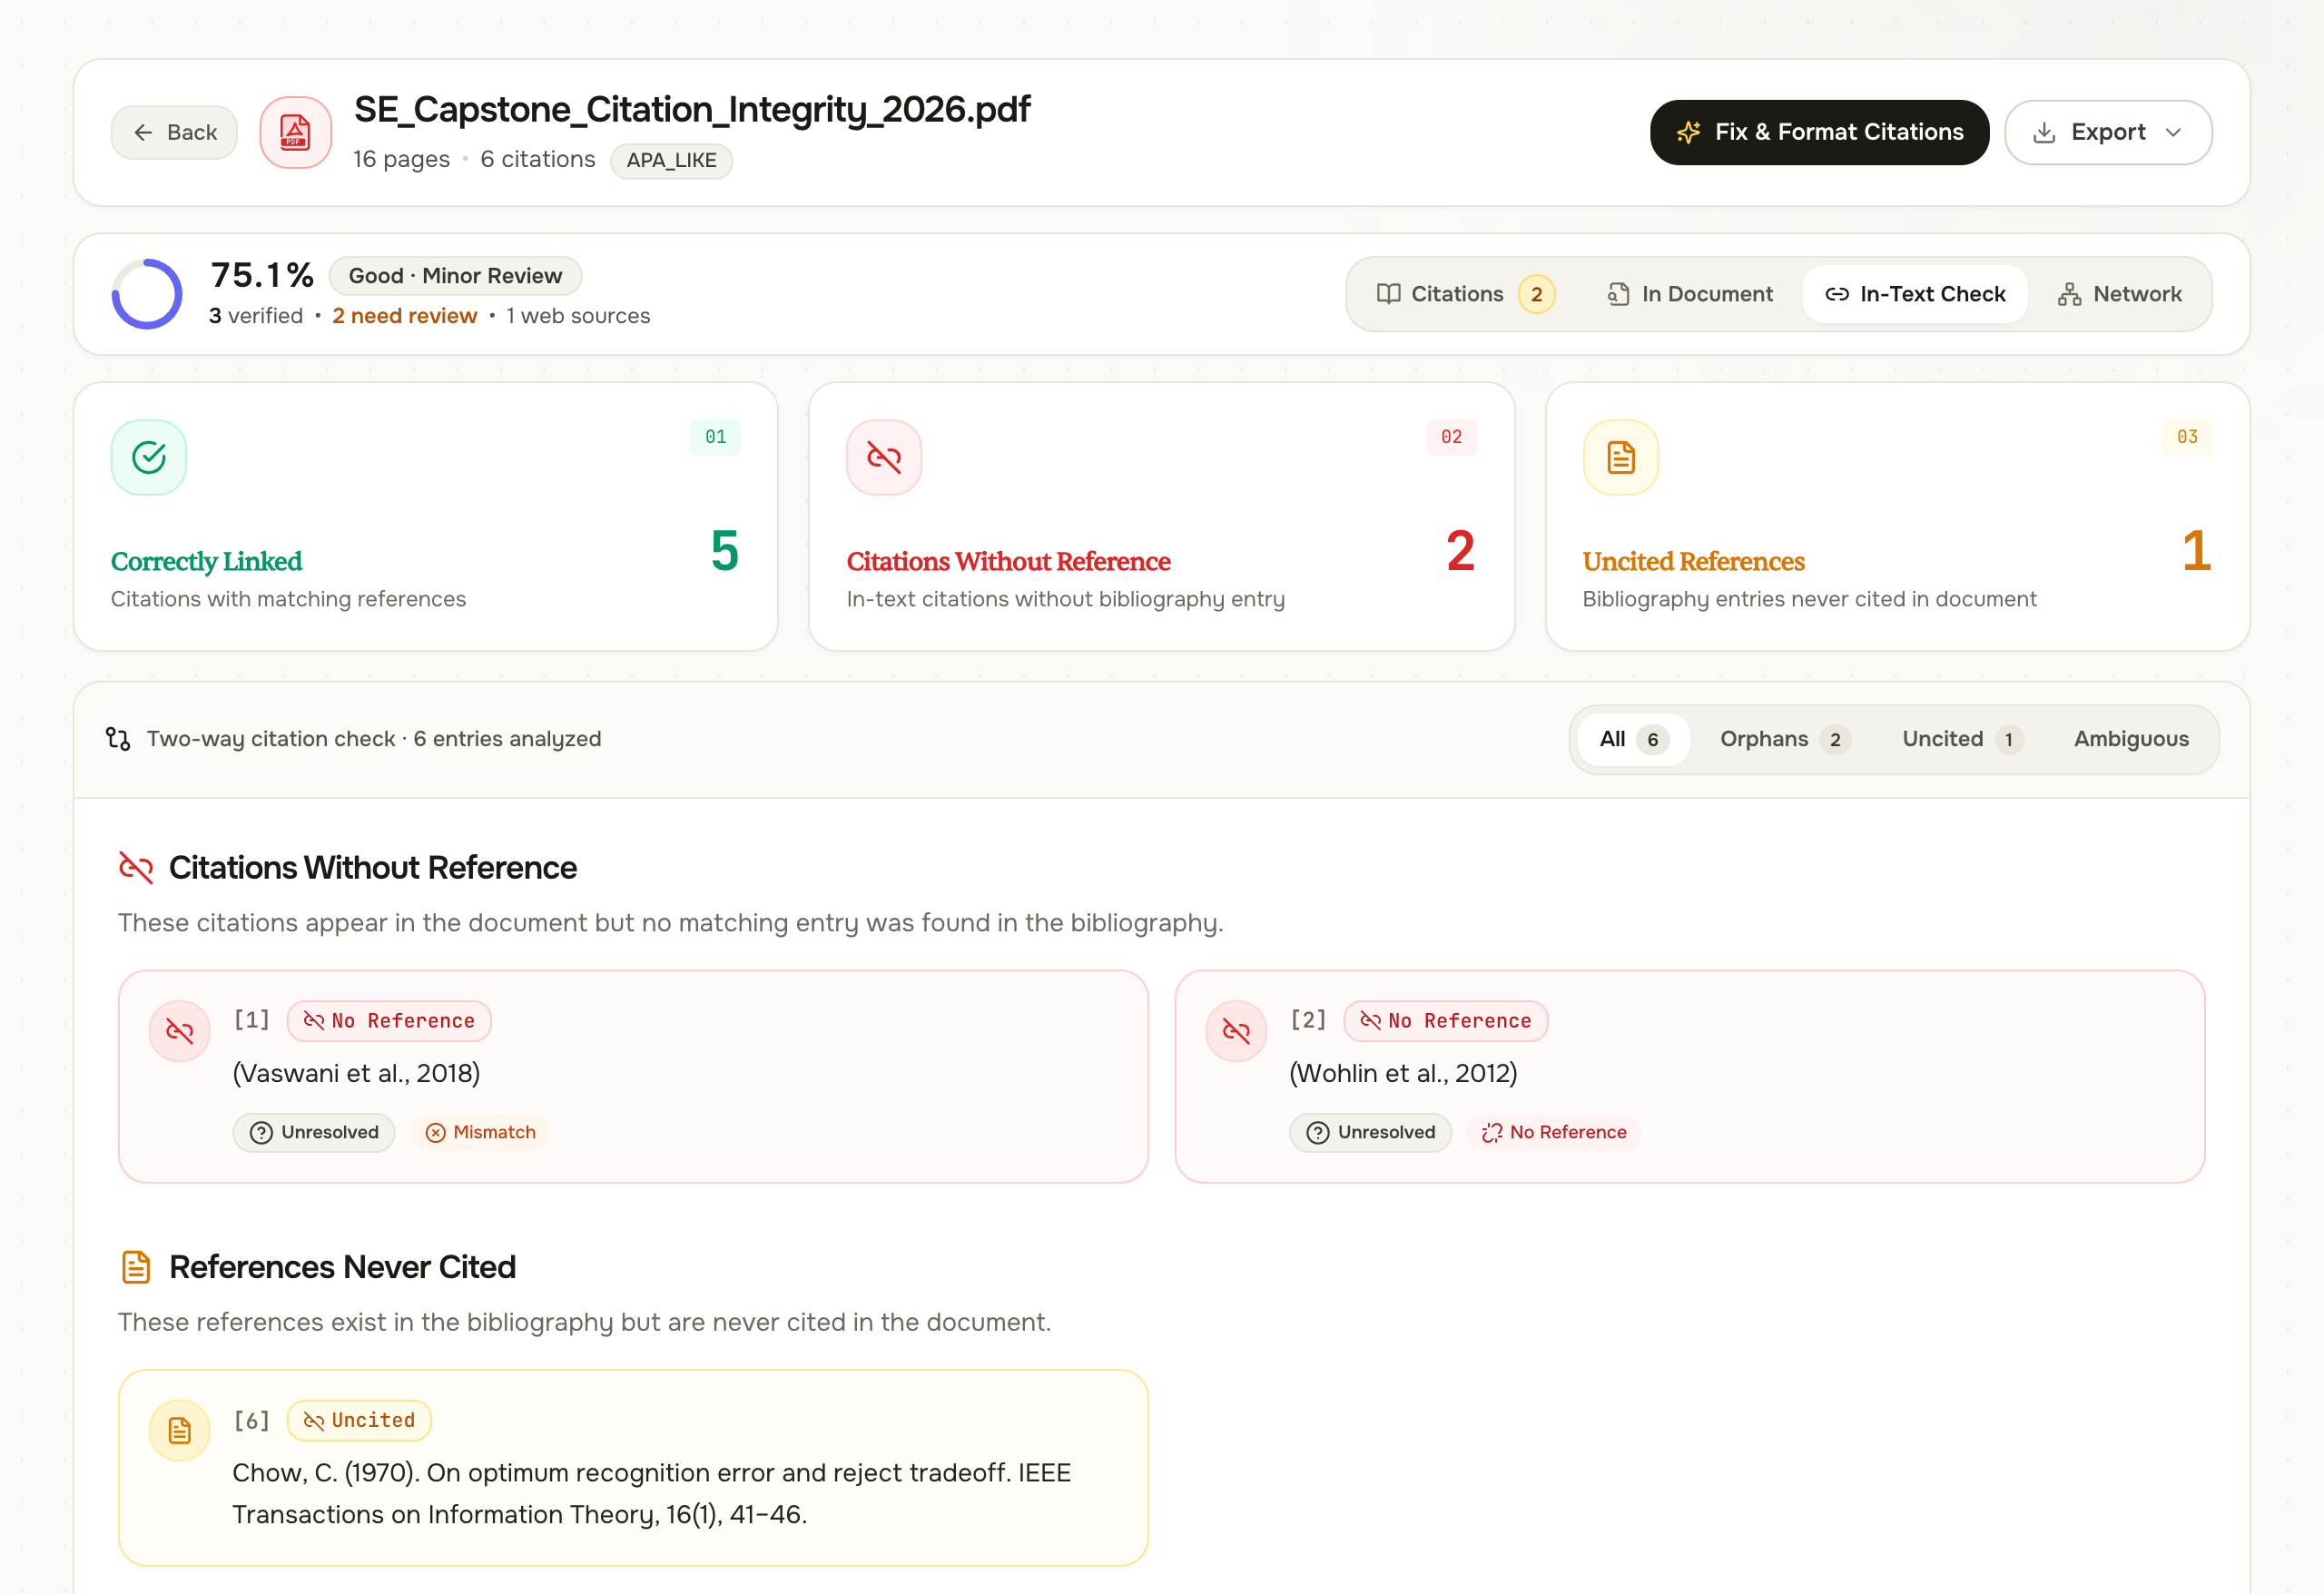
\includegraphics[width=0.84\textwidth,keepaspectratio]{picture/figures/08-consistency-check.png}
    \caption[Bidirectional In-Text Consistency view isolating orphan citations and uncited entries]{Bidirectional In-Text Consistency view (\texttt{/verification/report/\{id\}/consistency}) separating matched citations from orphan inline markers and uncited bibliography entries.}
    \label{fig:demo-consistency}
\end{figure}

\rqanswer{RQ4}{CITRA generalizes across disciplines and document formats, achieving $100.00\%$ ($120/120$) accuracy across six domains and seven styles on raw references, $97.7\%$--$100.0\%$ bibliography detection across 310 PDFs, and zero false hallucination flags on clean published manuscripts.}

\section{RQ5: Latency, Caching Efficiency, and Concurrency Scalability}
\label{sec:nfr-benchmarks}

Figure~\ref{fig:nfr-scalability} and Tables~\ref{tab:nfr-step-latency}--\ref{tab:nfr-deadline-stress} report non-functional benchmarks executed via \texttt{scripts/\allowbreak benchmark\_pipeline\_performance.py}. Warm-cache end-to-end $P_{90}$ latency scales linearly from $0.58\text{\,s}$ (12-page article) to $1.33\text{\,s}$ (50-page capstone report, well within the $2.5\text{\,s}$ \texttt{NFR-01} target) and $4.22\text{\,s}$ (156-page monograph), with peak RSS bounded at $1{,}030.8\text{\,MB}$ ($\le 1.5\text{\,GB}$ \texttt{NFR-02} limit). Tier-0 FTS5 and GROBID caching accelerate retrieval by $688.72\times$ ($8{,}635.8\text{\,ms} \rightarrow 12.5\text{\,ms}$) and end-to-end processing by $19.41\times$ (Table~\ref{tab:nfr-cold-warm-cache}). Under 20 and 50 simultaneous student uploads (Table~\ref{tab:nfr-deadline-stress}), \texttt{PipelineAdmissionController} and SQLite WAL complete $50/50$ submissions ($100\%$) with zero database lock errors and zero HTTP 5xx/429 failures.

\begin{figure}[H]
    \centering
    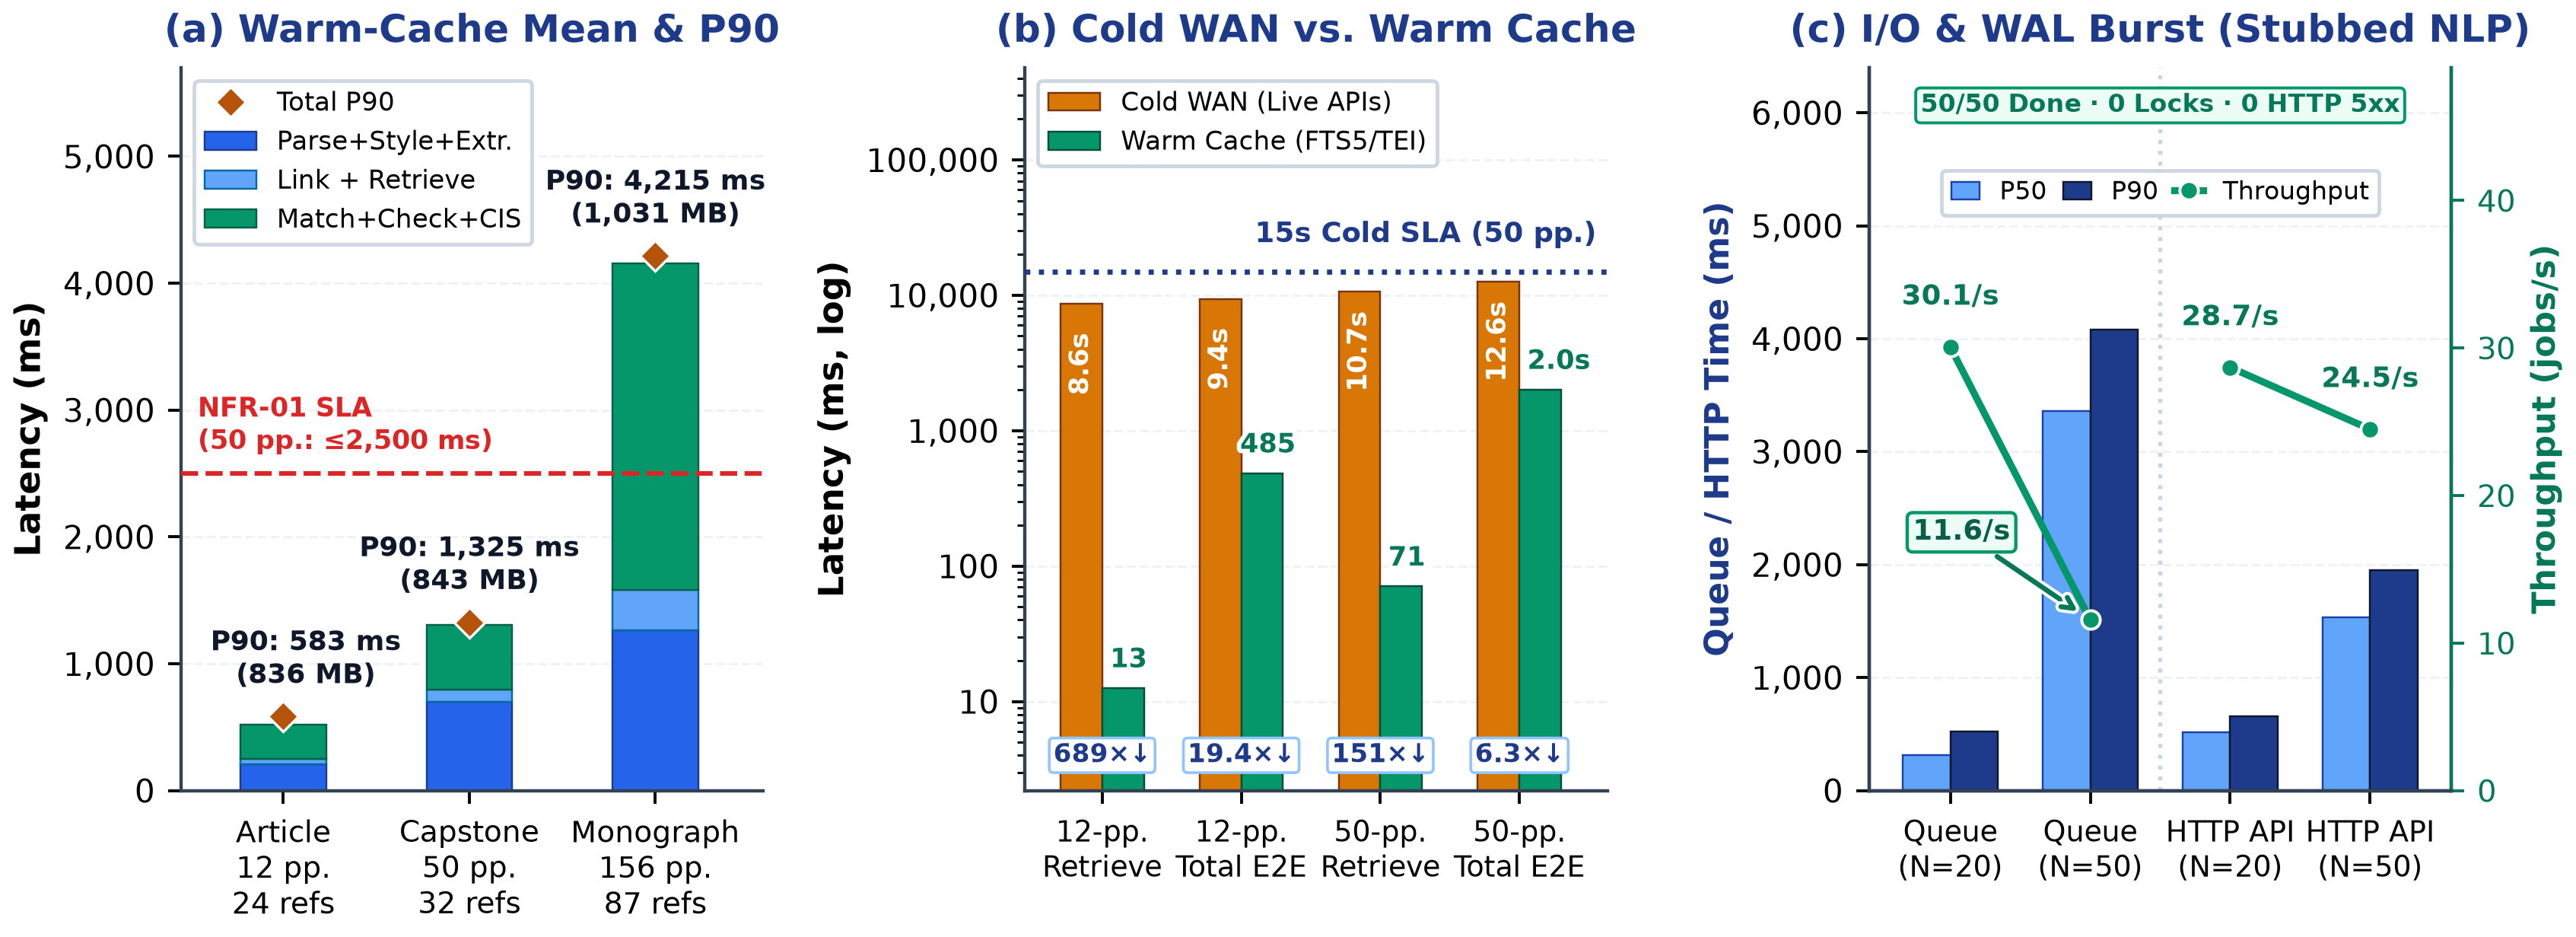
\includegraphics[width=\textwidth,keepaspectratio]{picture/figures/fig5_2_nfr_scalability.png}
    \caption[Pipeline stage latency, log-scale cache speedup, and 50-user concurrent burst throughput]{Systems performance and scalability plots: (a) per-stage warm-cache latency breakdown and RSS across manuscript scales relative to the \texttt{NFR-01} SLA ceiling, (b) log-scale cold WAN versus warm FTS5 cache latency, and (c) 20-user and 50-user concurrent burst latency and throughput.}
    \label{fig:nfr-scalability}
\end{figure}

{\setlength{\tabcolsep}{3.5pt}
\begin{longtable}{|L{0.22}|L{0.22}|C{0.11}|C{0.11}|C{0.11}|C{0.11}|C{0.12}|}
\caption{Warm-cache per-step latency percentiles and memory usage across three manuscript scales.}\label{tab:nfr-step-latency}\\
\hline
\textbf{Manuscript Scale} & \textbf{Stage} & \textbf{$P_{50}$ (ms)} & \textbf{$P_{90}$ (ms)} & \textbf{$P_{99}$ (ms)} & \textbf{Heap $\Delta$ (MB)} & \textbf{RSS (MB)} \\
\hline
\endfirsthead
\multicolumn{7}{c}{\itshape Table \thetable\ (continued from previous page)}\\
\hline
\textbf{Manuscript Scale} & \textbf{Stage} & \textbf{$P_{50}$ (ms)} & \textbf{$P_{90}$ (ms)} & \textbf{$P_{99}$ (ms)} & \textbf{Heap $\Delta$ (MB)} & \textbf{RSS (MB)} \\
\hline
\endhead
\hline
\multicolumn{7}{r}{\itshape Continued on next page}\\
\endfoot
\hline
\endlastfoot
\textbf{Article} (12\,pp., 24\,refs) & \texttt{parsing} + \texttt{extract} & 182.8 & 263.7 & 309.7 & 2.36 & 835.7 \\
 & \texttt{link} + \texttt{retrieve} & 39.6 & 48.0 & 52.5 & 0.18 & 835.7 \\
 & \texttt{compare} + \texttt{check} & 268.3 & 274.5 & 276.4 & 0.22 & 835.7 \\
 & \textbf{Total (All 8 steps)} & \textbf{494.1} & \textbf{583.4} & \textbf{635.5} & \textbf{1.61} & \textbf{835.7} \\
\hline
\textbf{Capstone} (50\,pp., 32\,refs) & \texttt{parsing} + \texttt{extract} & 693.1 & 702.9 & 705.3 & 6.93 & 843.1 \\
 & \texttt{link} + \texttt{retrieve} & 98.9 & 100.4 & 101.0 & 0.32 & 843.2 \\
 & \texttt{compare} + \texttt{check} & 506.2 & 530.6 & 536.1 & 0.37 & 843.2 \\
 & \textbf{Total (All 8 steps)} & \textbf{1306.9} & \textbf{1325.1} & \textbf{1333.0} & \textbf{4.39} & \textbf{843.4} \\
\hline
\textbf{Monograph} (156\,pp., 87\,refs) & \texttt{parsing} + \texttt{extract} & 1257.4 & 1273.1 & 1276.2 & 16.78 & 1029.8 \\
 & \texttt{link} + \texttt{retrieve} & 317.0 & 320.8 & 322.2 & 0.38 & 1029.8 \\
 & \texttt{compare} + \texttt{check} & 2593.0 & 2633.8 & 2642.7 & 1.37 & 1029.9 \\
 & \textbf{Total (All 8 steps)} & \textbf{4159.7} & \textbf{4215.3} & \textbf{4215.6} & \textbf{11.10} & \textbf{1030.8} \\
\hline
\end{longtable}
}

{\setlength{\tabcolsep}{3.5pt}
\begin{longtable}{|L{0.27}|C{0.12}|C{0.12}|C{0.13}|C{0.13}|C{0.12}|C{0.11}|}
\caption{Cold-cache (live WAN APIs) versus warm-cache (TEI + SQLite FTS5) latency comparison.}\label{tab:nfr-cold-warm-cache}\\
\hline
\textbf{Cache Mode} & \textbf{Parse (ms)} & \textbf{Extr.\ (ms)} & \textbf{Retr.\ (ms)} & \textbf{Total (ms)} & \textbf{Retr.\ Gain} & \textbf{E2E Gain} \\
\hline
\endfirsthead
\multicolumn{7}{c}{\itshape Table \thetable\ (continued from previous page)}\\
\hline
\textbf{Cache Mode} & \textbf{Parse (ms)} & \textbf{Extr.\ (ms)} & \textbf{Retr.\ (ms)} & \textbf{Total (ms)} & \textbf{Retr.\ Gain} & \textbf{E2E Gain} \\
\hline
\endhead
\hline
\multicolumn{7}{r}{\itshape Continued on next page}\\
\endfoot
\hline
\endlastfoot
Cold Cache (Live WAN) & 76.2 & 243.1 & 8635.8 & 9407.6 & $1.00\times$ & $1.00\times$ \\
\hline
\textbf{Warm Cache (TEI + FTS5)} & 96.0 & \textbf{87.1} & \textbf{12.5} & \textbf{484.8} & \textbf{$688.72\times$} & \textbf{$19.41\times$} \\
\hline
\end{longtable}
}

{\setlength{\tabcolsep}{3pt}
\begin{longtable}{|L{0.22}|C{0.08}|C{0.16}|C{0.20}|C{0.19}|C{0.15}|}
\caption{Concurrent deadline burst tests on the admission queue and FastAPI HTTP multipart endpoint.}\label{tab:nfr-deadline-stress}\\
\hline
\textbf{Stress Scenario} & \textbf{$N$} & \textbf{Completed} & \textbf{Upload / Queue $P_{50}/P_{90}$ (ms)} & \textbf{Throughput} & \textbf{DB Lock / 5xx} \\
\hline
\endfirsthead
\multicolumn{6}{c}{\itshape Table \thetable\ (continued from previous page)}\\
\hline
\textbf{Stress Scenario} & \textbf{$N$} & \textbf{Completed} & \textbf{Upload / Queue $P_{50}/P_{90}$ (ms)} & \textbf{Throughput} & \textbf{DB Lock / 5xx} \\
\hline
\endhead
\hline
\multicolumn{6}{r}{\itshape Continued on next page}\\
\endfoot
\hline
\endlastfoot
Admission Queue Worker & 20 & \textbf{20 / 20} & 315.5 / 520.7 & \textbf{30.07 essays/s} & \textbf{0 / 0} \\
\hline
Admission Queue Worker & \textbf{50} & \textbf{50 / 50} & 3361.1 / 4079.2 & 11.57 essays/s & \textbf{0 / 0} \\
\hline
HTTP \texttt{POST /api/essays} & 20 & \textbf{20 / 20} & 514.2 / 659.4 & \textbf{28.68 req/s} & \textbf{0 / 0} \\
\hline
HTTP \texttt{POST /api/essays} & \textbf{50} & \textbf{50 / 50} & 1530.2 / 1948.0 & 24.49 req/s & \textbf{0 / 0} \\
\hline
\end{longtable}
}

\rqanswer{RQ5}{CITRA processes a 50-page capstone report in $1.33\text{\,s}$ ($P_{90}$ warm-cache; $9.41\text{\,s}$ cold WAN) within a $1.03\text{\,GB}$ peak RAM budget, achieves a $19.41\times$ warm-cache speedup, and sustains 50 simultaneous uploads with zero SQLite lock or HTTP 5xx errors.}

\section{Threats to Validity}
\label{sec:difficulties}

Following Wohlin et al.~\cite{wohlin2012experimentation}, four categories of methodological threats to validity are analyzed below.

\subsection{Internal Validity}

Because no human-annotated corpus of $10^5$ naturally occurring citation hallucinations exists publicly, the 120,000-sample benchmark uses programmatic perturbations of real papers. A potential threat is that synthetic perturbations could introduce shortcut artifacts. This threat was mitigated by partitioning base papers strictly before perturbation ($0\%$ ID/title overlap), ensuring non-zero Sentence-BERT scores across all four classes ($P(\texttt{verified} \mid \text{score} > 0) = 54.06\%$), forbidding \texttt{np.clip} feature truncation, splicing real authors and titles from the same research domain, and validating the exact same model weights on 120 unperturbed raw references and 310 real PDFs.

\subsection{External Validity}

The offline FTS5 database (\texttt{local\_papers.db}) consists primarily of computer science and NLP papers ($98.42\%$ ACL Anthology). Consequently, offline-only mode has lower recall on biomedical, humanities, or economics papers. In connected deployments, \textbf{CITRA} mitigates this domain skew by routing queries dynamically across 15+ multidisciplinary APIs (Crossref, OpenAlex, Europe PMC, NCBI/bioRxiv, DOAJ, DataCite, OpenLibrary, and \texttt{VNLegalVerifier}), confirmed by the $100.00\%$ result across six disciplines in \textbf{RQ4}.

\subsection{Construct Validity}

Construct validity concerns whether evaluation metrics reflect real academic integrity needs. First, commercial publisher paywalls often hide full article text and occasionally omit public abstracts; when an inline claim cites a specific table inside a paywalled body section absent from the abstract, sentence-level abstract alignment cannot verify or refute that detail. Second, CIS rubric weights represent an institutional grading policy rather than physical constants, although simplex sensitivity testing confirmed high rank stability ($\rho = 0.9987$).

\subsection{Conclusion Validity}

To guard against Type I errors from multiple baseline comparisons and skewed error distributions, all accuracy comparisons used paired continuity-corrected McNemar tests with Holm--Bonferroni family-wise error control ($\alpha = 0.05$), 1,000-resample paired bootstrap confidence intervals, and exact Clopper--Pearson binomial bounds for zero-count cells.

\section{Chapter Summary}

This chapter verified \textbf{CITRA} (\texttt{v3.90.7}) across 2,920+ automated checks, a full Requirements Traceability Matrix, and five empirical research questions, demonstrating $99.67\%$ in-distribution accuracy ($\text{ECE} = 0.0405$), $99.96\%$ OOD symbolic accuracy, $100.00\%$ six-domain E2E gold accuracy, and zero-error 50-user burst scalability. Chapter~\ref{chap:conclusion} summarizes achievements, current limitations, and future research directions.
